%%%%%%%%%%%%%%%%%%%%%%%%%%%%%%%%%%%%%%%%%
% Simple Sectioned Essay Template
% LaTeX Template
%
% This template has been downloaded from:
% http://www.latextemplates.com
%
% Note:
% The \lipsum[#] commands throughout this template generate dummy text
% to fill the template out. These commands should all be removed when 
% writing essay content.
%
%%%%%%%%%%%%%%%%%%%%%%%%%%%%%%%%%%%%%%%%%

%----------------------------------------------------------------------------------------
%	PACKAGES AND OTHER DOCUMENT CONFIGURATIONS
%----------------------------------------------------------------------------------------

\documentclass[12pt]{article} % Default font size is 12pt, it can be changed here

\usepackage{geometry} % Required to change the page size to A4
\geometry{a4paper} % Set the page size to be A4 as opposed to the default US Letter

\usepackage[utf8]{inputenc}

\usepackage{mathpazo} % Use the Palatino font
\usepackage[T1]{fontenc} % Required for accented characters
\linespread{1.05} % Change line spacing here, Palatino benefits from a slight increase by default

\usepackage[protrusion=true,expansion=true]{microtype} % Better typography

\usepackage{graphicx} % Required for including pictures

\usepackage{hyperref} % For URLs

\hypersetup{%
    pdfborder = {0 0 0}
} % remove boxes around ToC

\usepackage{float} % Allows putting an [H] in \begin{figure} to specify the exact location of the figure
\usepackage{wrapfig} % Allows in-line images such as the example fish picture

\usepackage{lipsum} % Used for inserting dummy 'Lorem ipsum' text into the template

\linespread{1.2} % Line spacing

%\setlength\parindent{0pt} % Uncomment to remove all indentation from paragraphs

% \graphicspath{{Pictures/}} % Specifies the directory where pictures are stored

\begin{document}

%----------------------------------------------------------------------------------------
%	TITLE PAGE
%----------------------------------------------------------------------------------------

\begin{titlepage}

\newcommand{\HRule}{\rule{\linewidth}{0.7mm}} % Defines a new command for the horizontal lines, change thickness here

\center % Center everything on the page

\textsc{\LARGE University of Milan}\\[1.5cm] % Name of your university/college
\textsc{\Large Project Report}\\[0.5cm] % Major heading
\textsc{\large Web \& Mobile Programming}\\[0.5cm] % Minor heading

\HRule \\[1.0cm]
{ \huge \bfseries Twitter Automa}\\[0.4cm] % Title of your document
\HRule \\[1.5cm]
\vspace{2mm} %2mm vertical space
 
\large \emph{Author:} Andrei \textsc{Ciulpan} % Your name
\\[0.3cm]
\large \emph{Badge Number:} 872394    % Badge number
\\[0.3cm]
\large \emph{Academic Year:} 2018-2019    % Academic Year
\\[0.3cm]
\large \emph{APP website:} \url{https://unimitwitterbot.herokuapp.com}   % Website
 
\vfill % Fill the rest of the page with whitespace

{\large Exam session of October 29, 2018}\\[3cm] % Date, change the \today to a set date if you want to be precise

%\includegraphics{Logo}\\[1cm] % Include a department/university logo - this will require the graphicx package


\end{titlepage}

%----------------------------------------------------------------------------------------
%	TABLE OF CONTENTS
%----------------------------------------------------------------------------------------

\tableofcontents % Include a table of contents

\newpage % Begins the essay on a new page instead of on the same page as the table of contents 

%----------------------------------------------------------------------------------------
%	INTRODUCTION
%----------------------------------------------------------------------------------------

\section{Introduction} % Major section

This is a project based on the Twitter APIs for the Web Programming course.
\newline
The purpose of this project is to make an app using programming and markup languages designed for web technology such as HTML/CSS/JavaScript.
\newline
This app automatically tweets out random hashtags that are in the current global trending list
and provides, for each tweet, some additional information like the number of retweets, favorites, tweet ID and date of
creation (this information is updated automatically via a webhook connection with Twitter).
This app was developed locally and then deployed to a cloud platform as a service (PaaS) called Heroku which supports several
programming languages like NodeJS, an open-source, cross-platform JavaScript run-time environment that executes code 
outside of a browser, which I used to run server-side scripts on the cloud platform.

%------------------------------------------------

\subsection{Project Analysis} % Sub-section

The following sub-sections will describe some aspects of this application such as users (who the app is meant for), business model and
data flow. The technological aspects will be shown in section 2.

%------------------------------------------------


\subsubsection{Users} % Sub-sub-section

\textbf{Technical capabilities and possibilities}
\\[0.3cm]
This app is designed for any user who knows how to use Twitter and a browser on a very basic level; the user 
should be capable of understanding what a tweet or a trending hashtag is and how to access a website through a browser.
Anyone can connect to the website through a browser, therefore the only limitation of this app is that the device used by the user
must be able to connect to the internet and display HTML content (for example through a browser). 
The information is displayed entirely in text, which means that the users won't use a lot of bandwidth to access the website.
\pagebreak

\noindent \textbf{Languages}
\\[0.3cm]
The website is displayed in the english language, therefore the user must understand basic english
in order to be able to understand the contents.
\\[0.3cm]
\textbf{Motivation}
\\[0.3cm]
The app's only purpose is to provide free information on an entertainment level for users interested
in the global trending hashtags on Twitter.
 

%------------------------------------------------


\subsubsection{Business Model} % Sub-sub-section

The business model of this app is completely free: there will be no ads or content locked
behind a subscription fee therefore it has no real value except for it being a source of information for interested users.


%------------------------------------------------


\subsubsection{Data Flow} % Sub-sub-section

\textbf{Obtaining the data}
\\[0.3cm]
The data displayed on the website is automatically updated via a webhook connection with Twitter. What this means is that every 
time something happens on the bot's Twitter account, for example when one of its tweets gets a favorite (like)
the information on the website is updated through a method called getTweets that will be explained in a later section.
\newline
Note that in the picture below (Figure 1)  it took roughly 1.2 ms to get 
the tweets that the bot made so far from its own Twitter account and update the list which is then passed to the client where it is formatted and displayed
in a human readable manner.
It can be concluded that the time it takes to update the list is very insignificant and the user will not even notice it.

\begin{figure}[H] % Example image
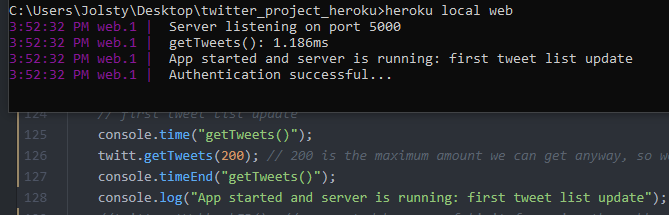
\includegraphics[width=1\linewidth]{images/getTweetsTime}
\caption{Time to get tweet list from Twitter by using the APIs.}
\label{getTweetsTime}
\end{figure}

\noindent\textbf{Archiving the data}
\\[0.3cm]
All the data shown on the website is received from the Twitter APIs by sending a GET request to statuses/user\_timeline.
Each call to this URL returns a JSON object (Figure 2) that represents metadata for multiple tweets from the caller's account and that we can handle with JavaScript.

\begin{figure}[H] % Example image
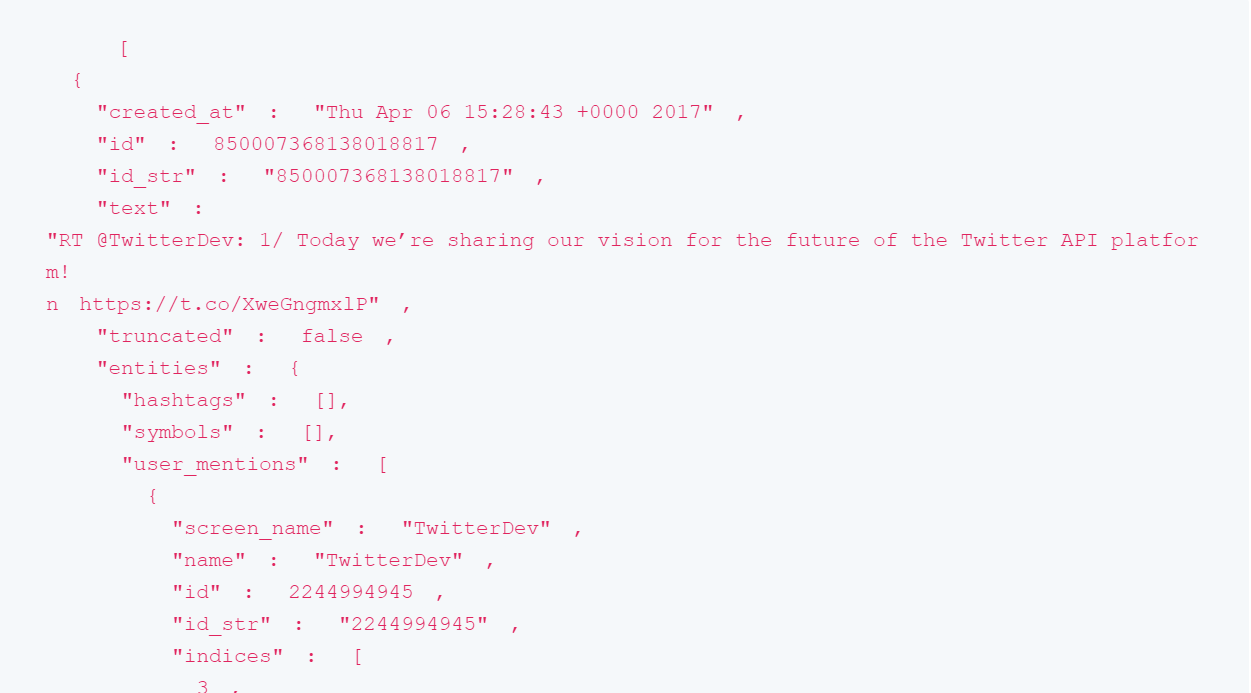
\includegraphics[width=1\linewidth]{images/getStatusesTimeline}
\caption{Data returned as a JSON object.}
\label{getStatusesTimeline}
\end{figure}

\noindent This JSON object is rather large, and there's no need to use every single piece of information inside of it.
The piece of code in Figure 3 makes sure to select only the necessary information like the tweet ID, number of retweets and so on.

\begin{figure}[H] % Example image
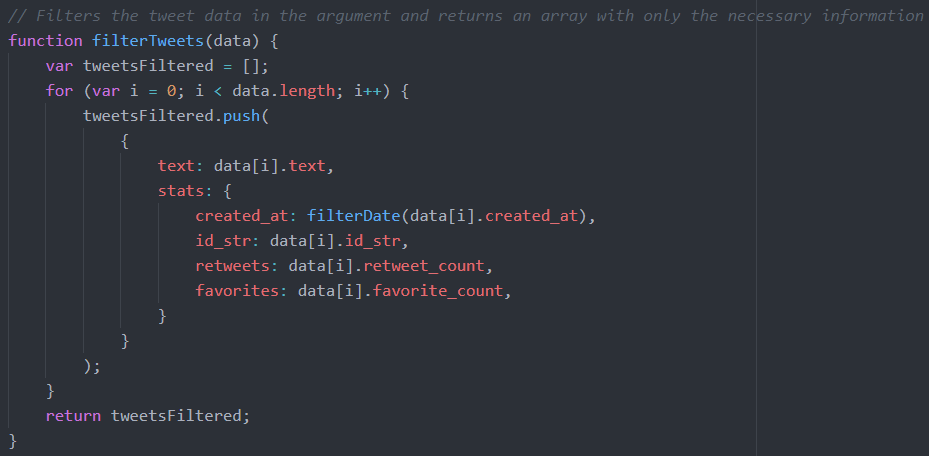
\includegraphics[width=1\linewidth]{images/informationSelection}
\caption{Selection of only the necessary information.}
\label{informationSelection}
\end{figure}

\noindent At the end of the day we are left with an array that contains selected information for multiple tweets.
All of this is done server-side, but now this data must be sent to the client in order to show it on the website.
\\[0.3cm]
\noindent\textbf{Showing the information on the website}
\\[0.3cm]
\noindent The data from the server is sent to the client by using a HTML div with the hidden display property as in Figure 4.
Normally there would be security issues by doing it this way but this data is not sensitive so it's not important.
This is done thanks to the Express and EJS modules but they will be explained later on.

\begin{figure}[H] % Example image
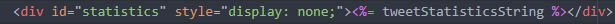
\includegraphics[width=1\linewidth]{images/statisticsDiv}
\caption{Passing data from server to client.}
\label{statisticsDiv}
\end{figure}

\noindent Then we get this data in a client-side script and add some HTML rules so it's interpreted
nicely by the browser (Figure 5). You can see in the first line of code that we get the hidden div shown before.

\begin{figure}[H] % Example image
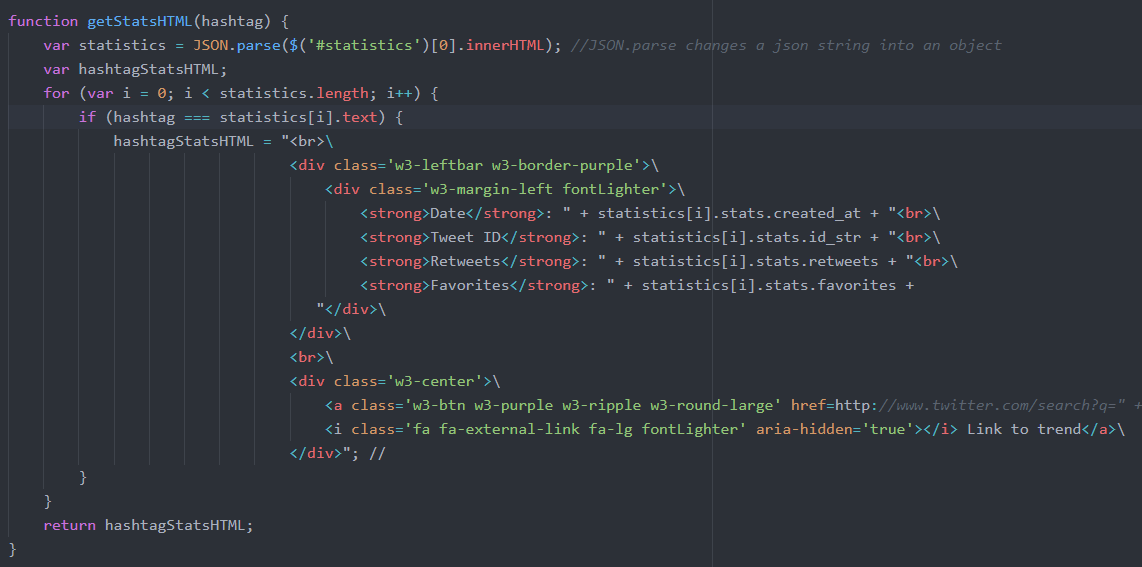
\includegraphics[width=1\linewidth]{images/interpretingTweetStatistics}
\caption{Adding some HTML rules to our data.}
\label{interpretingTweetStatistics}
\end{figure}

\noindent This is done everytime a button that shows additional information is clicked.
In Figure 6 you can see how it has a small impact on performance (roughly 0.4 ms).

\begin{figure}[H] % Example image
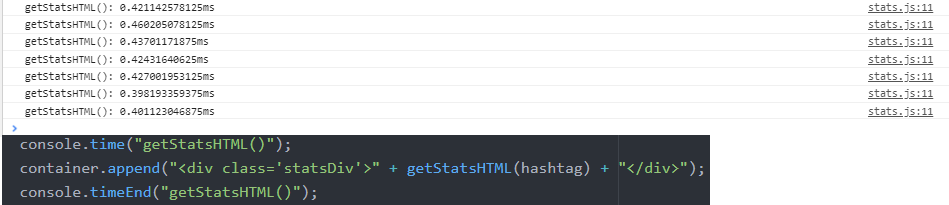
\includegraphics[width=1\linewidth]{images/getStatsHTMLTime}
\caption{Time to get tweet list from Twitter by using the APIs.}
\label{getStatsHTMLTime}
\end{figure}


%----------------------------------------------------------------------------------------
%	MAJOR SECTION 
%----------------------------------------------------------------------------------------

\section{Technological Aspects} 

\subsection{MVC}
\noindent The app follows an MVC pattern. The Model-View-Controller is an architectural pattern that separates an 
application into three main logical components: the model, the view, and the controller.
 Each of these components are built to handle specific development aspects of an application.
\newline
The Model component corresponds to all the data-related logic that the user works with. In this case the model represents
the data in the form of an array of JSON objects (usually the model is the database, but we don't use that in this project) 
that is being transferred between the view and the controller, therefore it is the object that we pass
from server to client. 
\newline
The View component is used for all the UI logic of the application. In this case it represents how our information
is displayed on the website. It's basically our HTML/CSS code.
The app also uses a template engine called EJS. EJS is a simple templating language that lets you generate HTML markup with plain JavaScript.
The way it was used in this app can be seen in Figure 7.
We have to set EJS as the view engine for our Express application using app.set('view engine', 'ejs');.
Notice how we send a view to the user by using res.render(). It is important to note that res.render() will look in a views folder for the view. 
So we only have to define "index"  since the full path is views/index.ejs.

\begin{figure}[H] % Example image
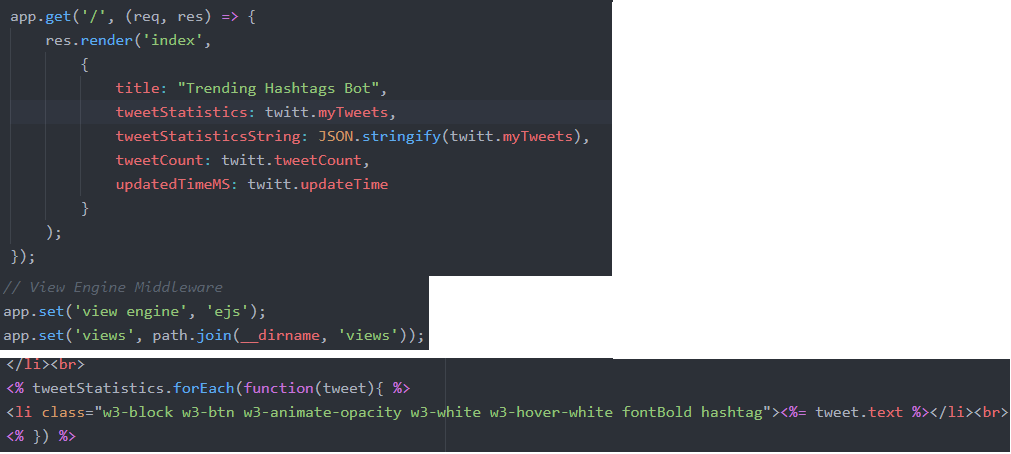
\includegraphics[width=1\linewidth]{images/EJS}
\caption{EJS}
\label{EJS}
\end{figure}

\noindent The Controller accepts user input (for example visiting a website, clicking on a button or submitting a form) and converts it to commands for the model or view. In this case it can be what the user can do with it like, for example, on the website there's a button that the user can click on to show more information for a tweet as you can see in Figure 8.

\begin{figure}[H] % Example image
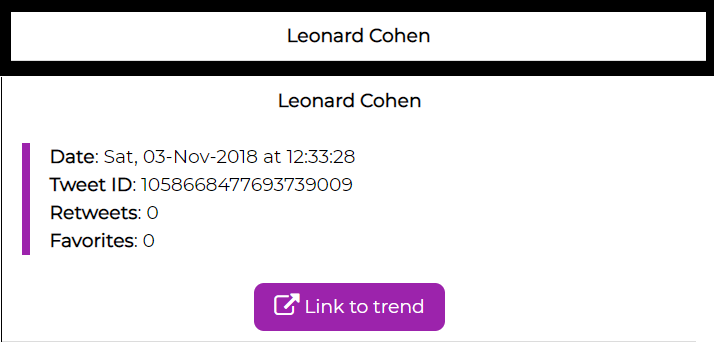
\includegraphics[width=1\linewidth]{images/hashtagButton}
\caption{Example of user input.}
\label{hashtagButton}
\end{figure}

\subsection{Used technologies}
\noindent This app uses all the technologies required by the professor, such as HTML5, CSS, JavaScript, AJAX, NodeJS and a cloud platform called Heroku. We will also go more in-depth into the Twitter APIs later.


  \subsubsection{HTML5  \cite{html5}} All pages are developed in valid HTML5 and they use the HTML5 APIs like, for example, the DOM which can be easily modified by JavaScript code (see Figure 9 for an example).

	\begin{figure}[H] % Example image
	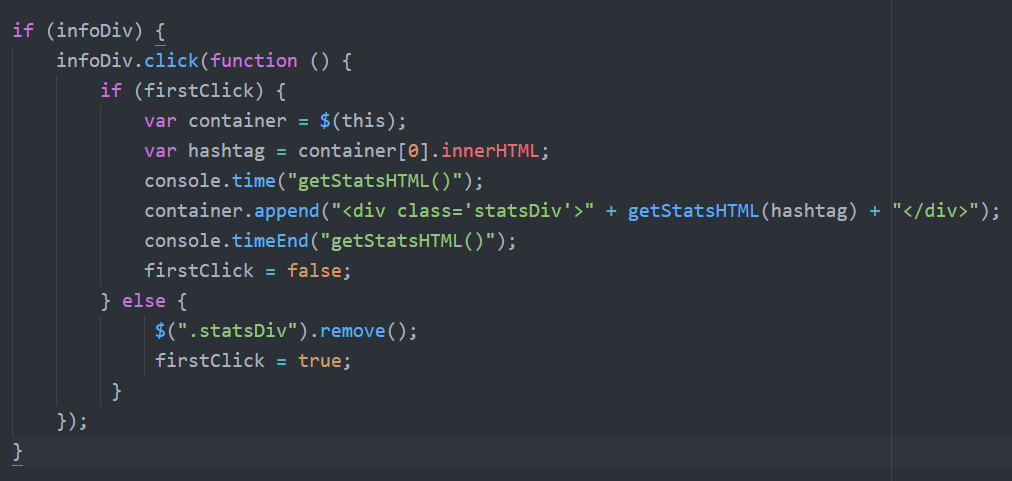
\includegraphics[width=1\linewidth]{images/htmlAPI}
	\caption{DOM manipulation using jQuery. When the button is clicked by the user, \$(this) takes it and appends another div to it so that it can expand.}
	\label{htmlAPI}
	\end{figure}

  \subsubsection{CSS \cite{css}} The presentation of the documents is styled by using CSS files embedded into the HTML files (see Figure 10 for an example).
	We can see that there are some third-party CSS files like fontawesome (which is used for some icons like the HOME button), w3.css and font.css. There's also a file called custom.css which I created.
 	Note that I didn't write all of my HTML5 \& CSS code because I used a free to use template from W3.CSS called Dark Portfolio which can be found here: 
	\url{https://www.w3schools.com/w3css/tryw3css_templates_dark_portfolio.htm}.

	\begin{figure}[H] % Example image
	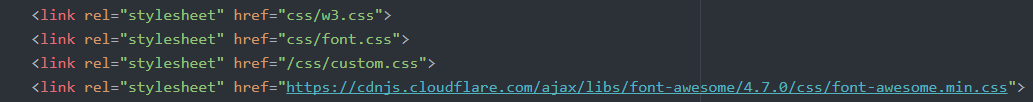
\includegraphics[width=1\linewidth]{images/embeddedCSS}
	\caption{Embedding CSS into HTML.}
	\label{embeddedCSS}
	\end{figure}

  \subsubsection{JavaScript \cite{javascript}} All client-side code is written in JavaScript using either vanilla JavaScript or jQuery.
	jQuery is a JavaScript library invented by John Resig, which is now maintained by a team of developers at the jQuery Foundation.
	The jQuery library makes front-end development easier by simplifing things such as Animations, AJAX Operations, DOM Manipulation, 
	Event Handling, and lot more. As a result, you can write fewer lines of code and accomplish more in a short amount of time.
	There have been a lot of performance tests (benchmarks) to actually see how much slower jQuery is than vanilla JavaScript. According to Marco Trombino, a front-end developer
	that tested a task that puts 10.000 new elements with a class inside a target element noticed that jQuery is moderately slower than vanilla JavaScript: 
	\textit{"As we could have expected Vanilla performed the task in 18,99 ms, whereas jQuery did it in 195,89 ms. Ten times faster."} \cite{jQuery}.
	As we can see, the only drawback of using jQuery is that it can be slower for very large and intensive projects, but obviously this is not the case for this relatively
	small project and the users won't even notice it. 

   \subsubsection{AJAX  \cite{ajax}} The app uses XMLHttpRequests (Figure 11) to POST form data to the server \cite{ajaxForms} (note that AJAX is the safest and most reliable way to make HTTP requests).
	AJAX is better than conventional ways to send form data because we can send the form without having to refresh the page (this means that the user is happy because the state
	of the page never changes) and the data will be sent in the background with an async request.

	\begin{figure}[H] % Example image
	\includegraphics[width=1\linewidth]{images/AJAX}
	\caption{Sending forms with AJAX.}
	\label{AJAX}
	\end{figure}

	\noindent As you can see this form is sent as a JSON string with a POST method on the "/message" URL. Our Express app then interprets this in NodeJS and logs the received data to console (Figure 12)

	\begin{figure}[H] % Example image
	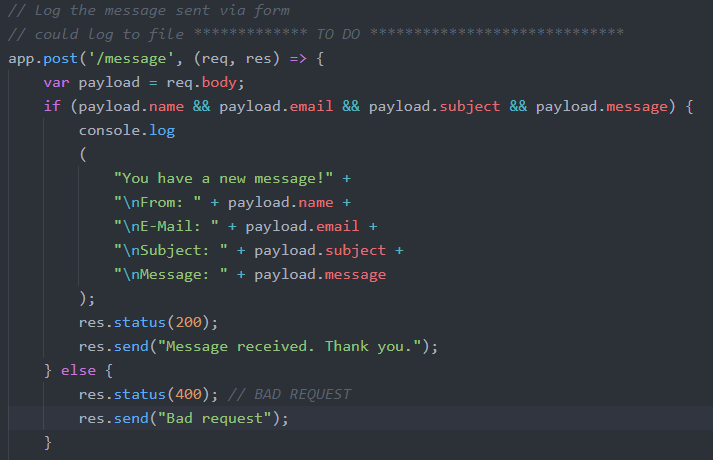
\includegraphics[width=1\linewidth]{images/AJAXserver}
	\caption{Receiving the form on the server.}
	\label{AJAXserver}
	\end{figure}

   \subsubsection{NodeJS  \cite{nodejs}} The app uses various NodeJS modules that must be installed (Figure 13) like Express, Body-Parser, Path and 2 other files that I wrote and included in the main app file.
	There's another module which is not shown in this image: const Twitter = require('twitter');.

	\begin{figure}[H] % Example image
	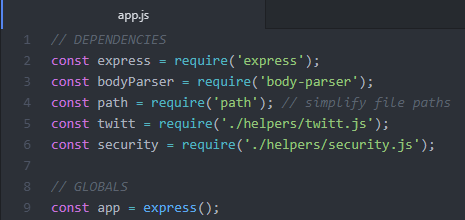
\includegraphics[width=1\linewidth]{images/NodeJS}
	\caption{NodeJS modules. The Express app object is created on line 9.}
	\label{NodeJS}
	\end{figure}

	\noindent Express \cite{express} is a minimal and flexible Node.js web application framework that provides a robust set of features for web and mobile applications.
	It facilitates the rapid development of Node based Web applications. Following are some of the core features of Express framework:
	1) Allows to set up middlewares to respond to HTTP Requests.
	2) Defines a routing table which is used to perform different actions based on HTTP Method and URL.
	3) Allows to dynamically render HTML Pages based on passing arguments to templates.
	\newline
	The app uses express to, among other things, handle routing (Figure 14): whenever an user makes a GET request to "/" then it renders a file called index.ejs (this is possible
	because, as pointed out earlier, the app uses EJS as a view engine) that sits inside the views directory.
	

	\begin{figure}[H] % Example image
	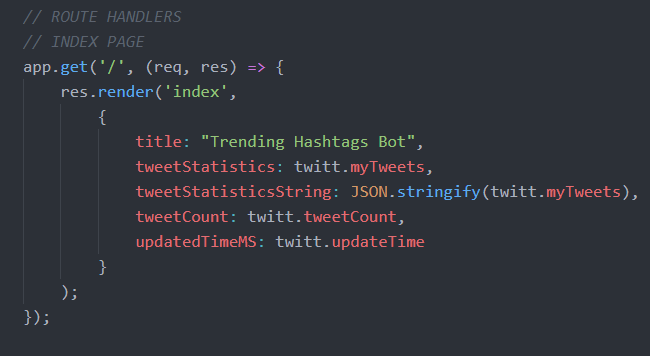
\includegraphics[width=1\linewidth]{images/express}
	\caption{Using the express framework.}
	\label{express}
	\end{figure}

	\noindent Another important thing that express is used for is to create a server that listens on a certain port (Figure 15).
	This is also possible with a module called "http" but express makes things a lot easier because it uses this module behind the scenes and provides additional abstraction.

	\begin{figure}[H] % Example image
	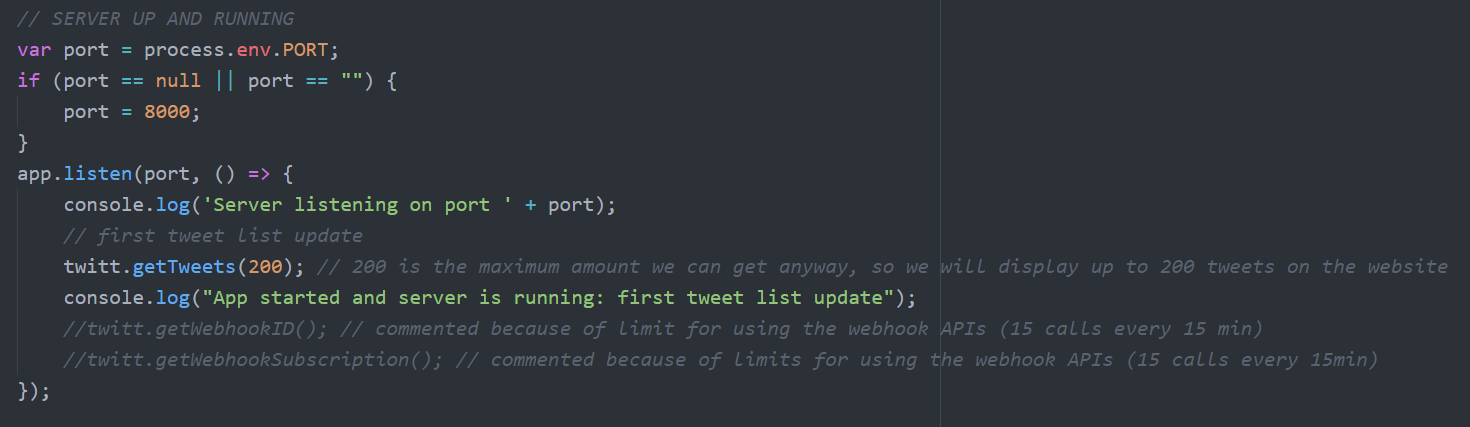
\includegraphics[width=1\linewidth]{images/expresslisten}
	\caption{Listening on a port with express.}
	\label{expresslisten}
	\end{figure}
 
	\noindent Body-Parser \cite{body-parser} parses incoming request bodies in a middleware before your handlers, available under the req.body property.
	The app uses this to parse JSON content so that, for example, it can read the form data sent through an AJAX call in POST (Figure 16).
	The second line of code in Figure 16  is a middleware and it parses UTF-8 encoded bodies. It helps to parse URL encoded data like JSON objects

	\begin{figure}[H] % Example image
	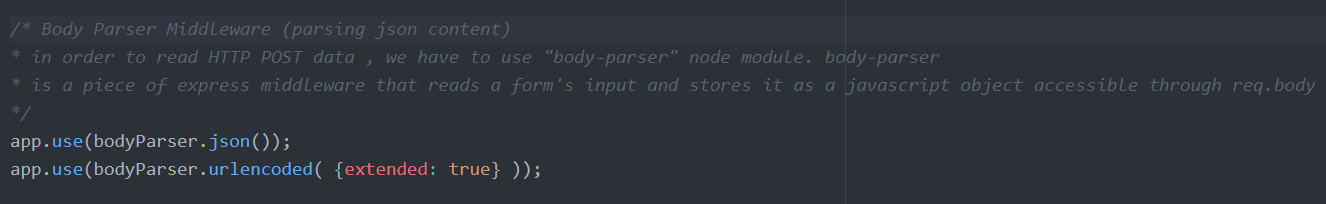
\includegraphics[width=1\linewidth]{images/bodyparser}
	\caption{Using the body-Parser module.}
	\label{bodyparser}
	\end{figure}

	\noindent Path \cite{path} provides utilities for working with file and directory paths. This app uses the path module to define a static directory for our files (Figure 17) that we can call root.
	The purpose of path.join(\_\_dirname, 'public') is to create an absolute path, using the directory where app.js is located as the base. In my example this piece of code will result in 
	C:/Users/Jolsty/Desktop/twitter\_project\_heroku/public. In conclusion, the line of code in Figure 17 will simply create an absolute path for the app.

	\begin{figure}[H] % Example image
	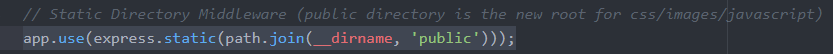
\includegraphics[width=1\linewidth]{images/pathStatic}
	\caption{Using the path module with an Express app.}
	\label{pathStatic}
	\end{figure}

	\noindent Twitter \cite{twitter} is an asynchronous client library for the Twitter REST and Streaming API's (Figure 18).
	This module is used to create a twitter object with the OAuth credentials. With this object it's possible to make requests to the Twitter APIs in a simple manner; we can, for example,
	make a GET request to "statuses/user\_timeline" which translates to \url{https://api.twitter.com/1.1/statuses/user\_timeline.json} which returns metadata for tweets on our 			account (Figure 2).
	We will go more in depth on this module on the next subsection to see how the app uses the APIs to get the necessary information from Twitter.

	\begin{figure}[H] % Example image
	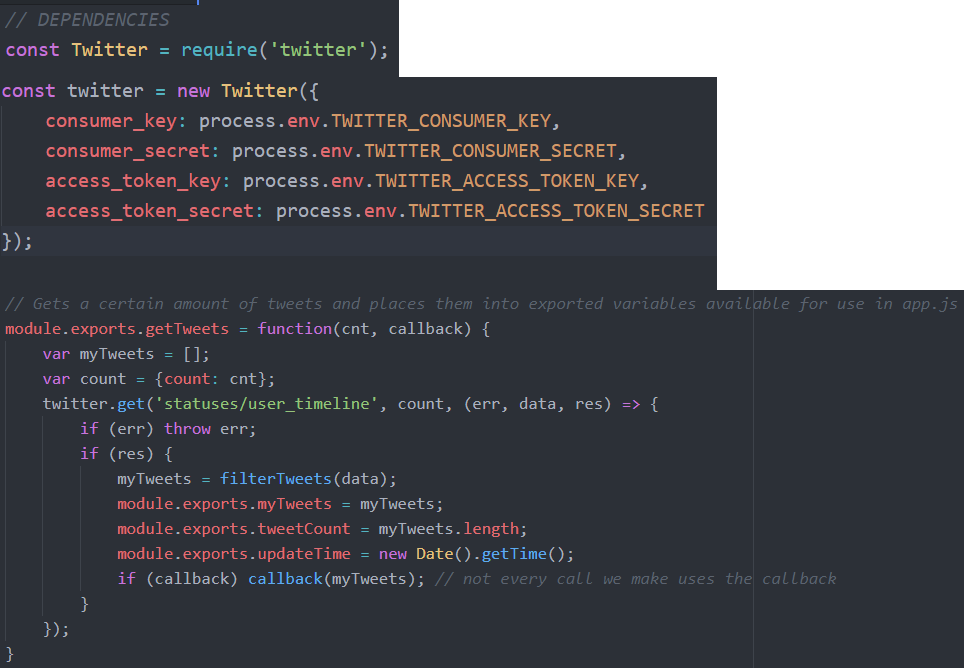
\includegraphics[width=1\linewidth]{images/twitter}
	\caption{Using the twitter module.}
	\label{twitter}
	\end{figure}

	 \subsubsection{Heroku \cite{heroku}}  Heroku is a platform as a service (PaaS) that enables developers to build, run, and operate applications entirely in the cloud.
	I specifically chose this platform because it's very easy to use and it allows for deploying Node apps.
	The deployment \cite{herokudeploy} works by pushing your code to a specific git repository (which is called heroku remote, unique for every heroku app). 
	Note that Heroku only deploys code that you push to the master branch of the heroku remote. Pushing code to another branch of the remote has no effect. After deployment, 			Heroku prepares the app for execution in a dyno - a smart container with a secure, curated Node stack.	


	\subsubsection{Twitter APIs  \cite{twitterAPI}}
	\noindent Twitter’s developer platform includes numerous API endpoints and tools to help build an app and solution on Twitter.
	Integrating with nearly all of the Twitter APIs requires the creation of a Twitter app and the generation of consumer keys and access tokens.
	There are many endpoints that we can call that return various interesting data in JSON format, but we are only interested in some of them:

	\begin{enumerate}
	
		\item Trends (Figure 19)

		\begin{figure}[H] % Example image
		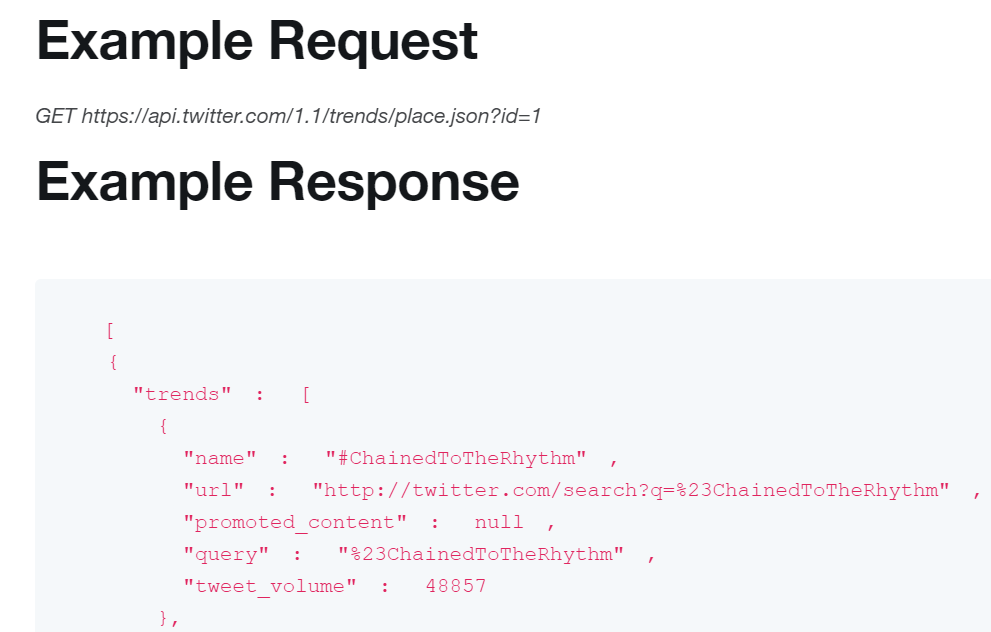
\includegraphics[width=1\linewidth]{images/trendsAPIv2}
		\caption{Trends endpoint.}
		\label{trendsAPIv2}
		\end{figure}

		This endpoint returns the top 50 trending topics for a specific WOEID \cite{woeid} (in our case the WOEID = 1 which represents the entire Earth), if trending information is 				available for it.
		The response is an array of trend objects that encode the name of the trending topic, the query parameter that can be used to search for the topic on Twitter Search, and 				the Twitter Search URL. This information is cached for 5 minutes. Requesting more frequently than that will not return any more data. As you can see in Figure 20 we call the 			getTrendsAndTweet() function every hour. This function gets the current trending list and then tweets out a single random one. The actual code that gets the trends and 				stores them in an array that is returned to a callback function is in Figure 21.

		\begin{figure}[H] % Example image
		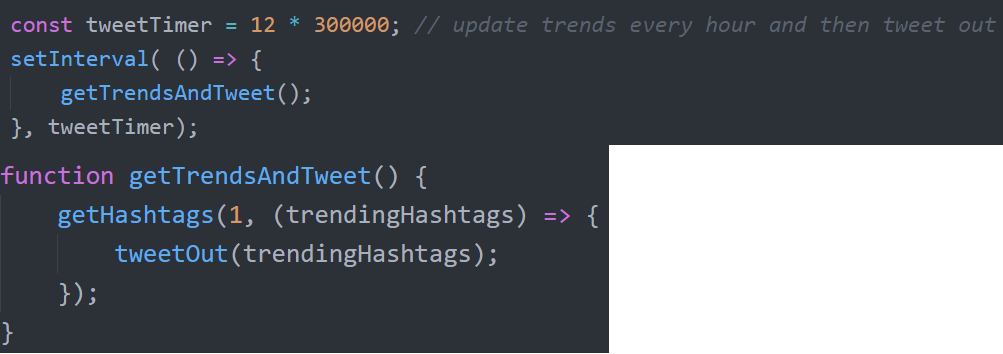
\includegraphics[width=1\linewidth]{images/trendsInterval}
		\caption{Updating trends every hour.}
		\label{trendsInterval}
		\end{figure}

		\begin{figure}[H] % Example image
		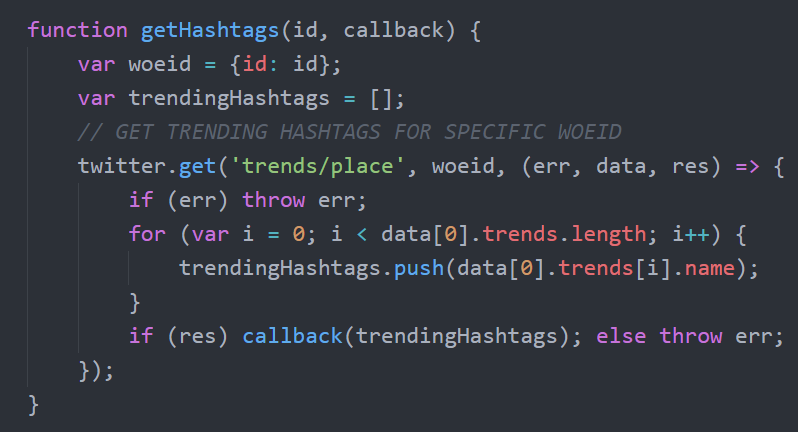
\includegraphics[width=1\linewidth]{images/trendsAPI}
		\caption{Using the trends endpoint (code).}
		\label{trendsAPI}
		\end{figure}
		
		\item Posting tweets (Figure 22)

		This endpoint updates the authenticating user’s current status, also known as Tweeting.
		For each update attempt, the update text is compared with the authenticating user’s recent Tweets. 
		Any attempt that would result in duplication will be blocked, resulting in a 403 error. A user cannot submit the same status twice in a row.

		\begin{figure}[H] % Example image
		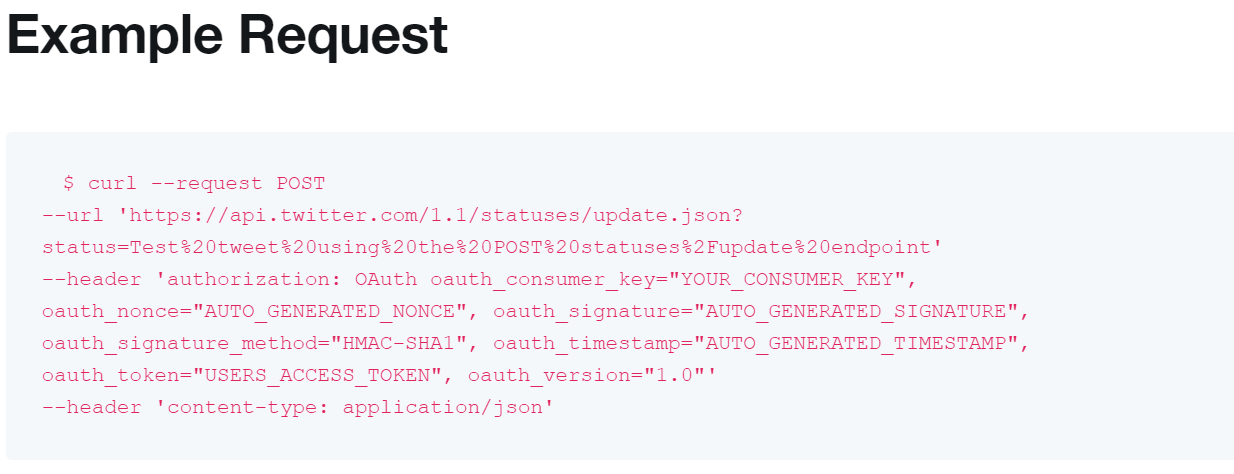
\includegraphics[width=1\linewidth]{images/tweetEndpoint}
		\caption{Post tweets endpoint. Remember that the authentication is managed by the twitter module.}
		\label{tweetEndpoint}
		\end{figure}

		The code that does the actual tweeting can be seen in Figure 23.

		\begin{figure}[H] % Example image
		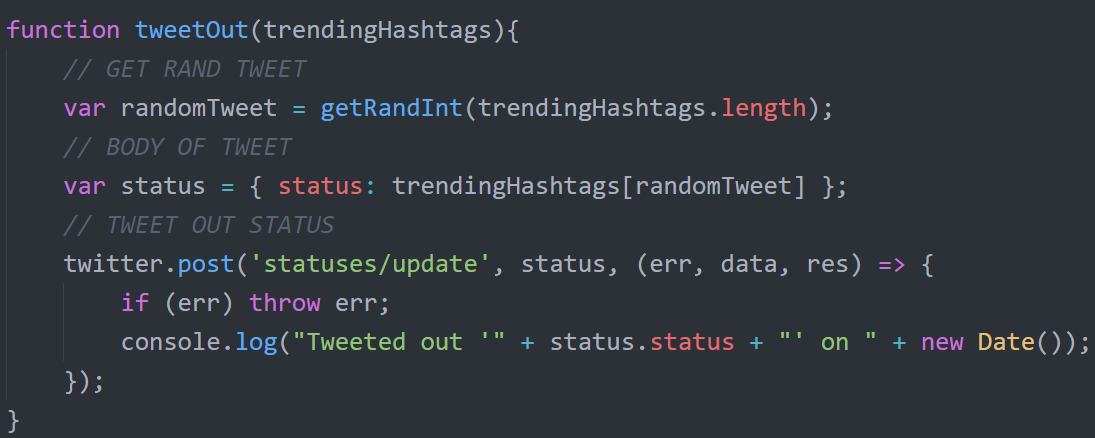
\includegraphics[width=1\linewidth]{images/tweetOut}
		\caption{Code to post tweets. The status is chosen randomly from the array of trends that is passed to the callback function in Figure 21.}
		\label{tweetOut}
		\end{figure}

		\item Getting tweet metadata (Figure 24)

		This endpoint returns a collection of the most recent tweets posted by the user indicated by the screen\_name or user\_id parameters.
		User timelines belonging to protected users may only be requested when the authenticated user either owns the timeline or is an approved follower of the owner.
		The timeline returned is the equivalent of the one seen as a user’s profile on twitter.com.
		This method can only return up to 3,200 of a user’s most recent tweets.

		\begin{figure}[H] % Example image
		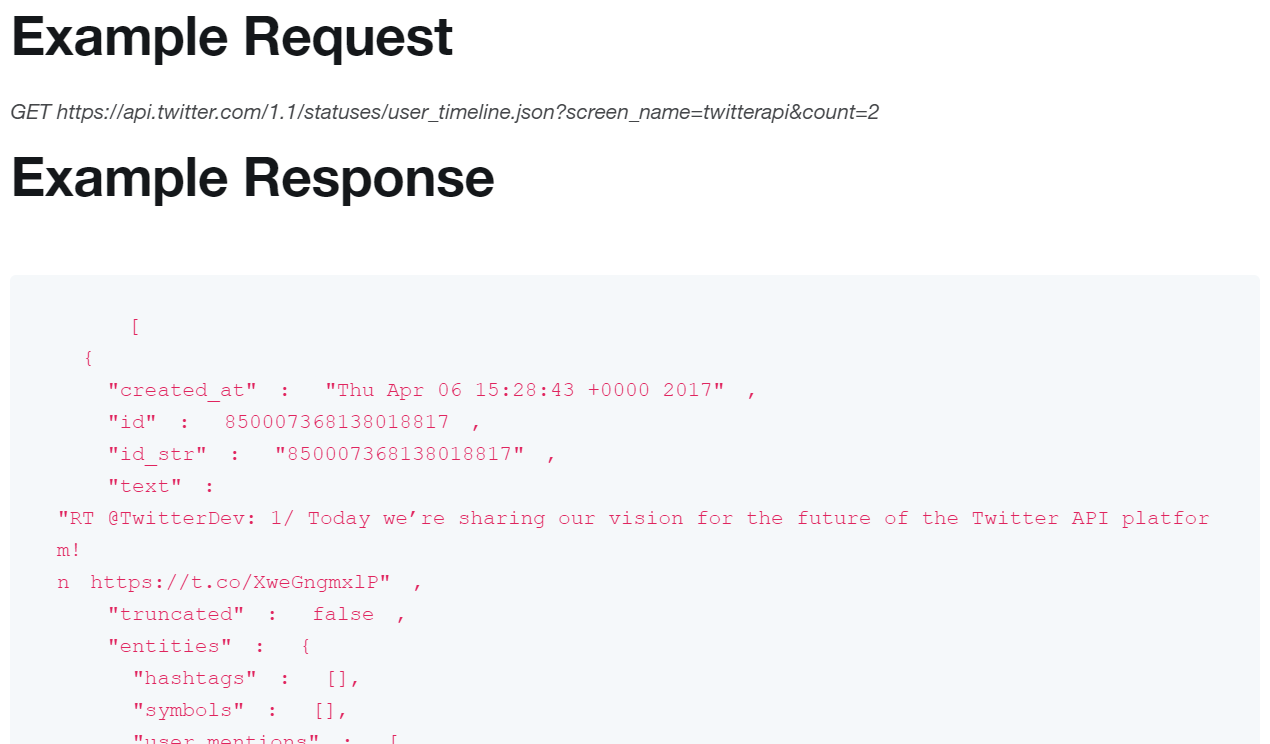
\includegraphics[width=1\linewidth]{images/getTweetEndpoint}
		\caption{Get tweets endpoint. Returns tweet metadata for the caller's account.}
		\label{getTweetEndpoint}
		\end{figure}

		In Figure 25 you can see the code to get the metadata. This function gets the recent tweets (the number is specified by the variable called cnt) from the account
		and, after filtering them through the filterTweets function, puts them in an exported variable that we can read from the main app.js file (this is so that we can render
		it for the client). We will also export a variable that holds the time when the list was updated and one to keep track of how many tweets were read (this can be different
		from the cnt variable because, for example, we can call this function with cnt = 200 but we don't actually have 200 tweets that can be returned).

		\begin{figure}[H] % Example image
		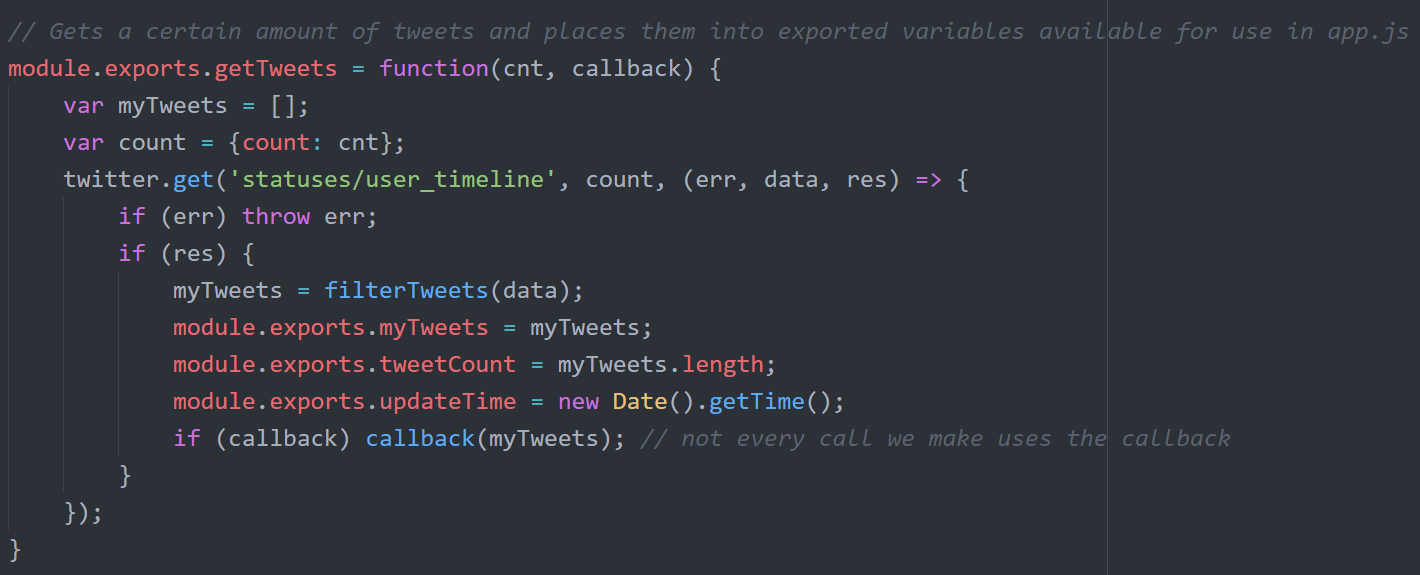
\includegraphics[width=1\linewidth]{images/getTweet}
		\caption{Code to get tweets metadata.}
		\label{getTweet}
		\end{figure}

		\item Account activity APIs (based on webhooks) \cite{webhooks}

		Webhooks are "user-defined HTTP callbacks". They are usually triggered by some event, such as pushing code to a repository or a comment being posted to a blog. 					When that event occurs, the source site makes an HTTP request to the URL configured for the webhook. Users can configure them to cause events on one site to invoke 				behaviour on another. The action taken may be anything. Common uses are to trigger builds with continuous integration systems or to notify bug tracking systems.					Since they use HTTP, they can be integrated into web services without adding new infrastructure. However, there are also ways to build a message queueing service on               		top of HTTP—some RESTful examples include IronMQ and RestMS. (source: Wikipedia)

		In the Summer of 2018 Twitter decided to replace (Figure 26) the usual streaming APIs with the Account Activity APIs,  a webhook-based API 
		that sends account events to a web app you develop, deploy and host.
		The Account Activity API provides you the ability to subscribe to realtime activities related to a user account via webhooks.
		This means that you can receive realtime Tweets, Direct Messages, and other account events from one or more of your owned or subscribed accounts 
		through a single connection. All activity types can be seen in Figure 27.
		\begin{figure}[H] % Example image
		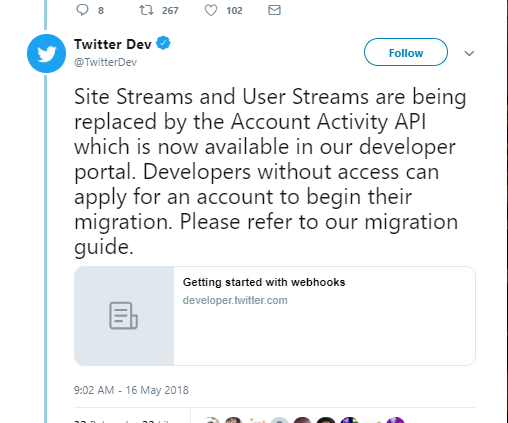
\includegraphics[width=0.7\linewidth]{images/deprecatedStream}
		\caption{Twitter replaces streaming APIs.}
		\label{deprecatedStream}
		\end{figure}

		\begin{figure}[H] % Example image
		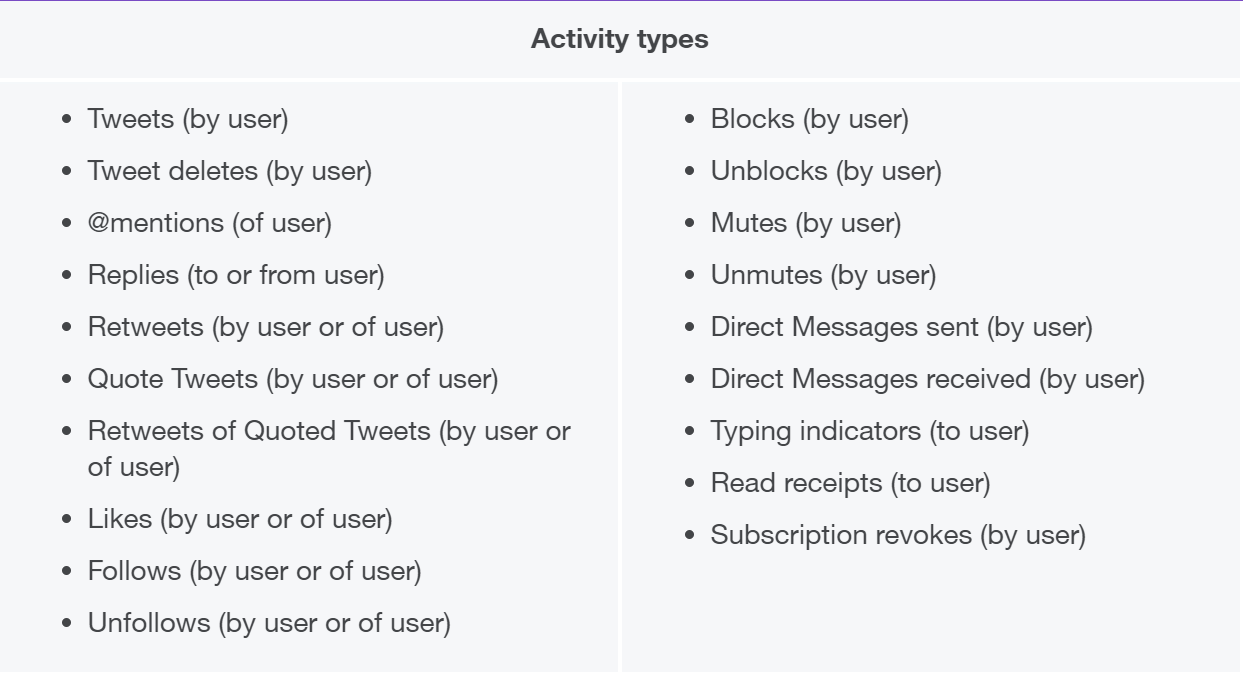
\includegraphics[width=1\linewidth]{images/activityAPIs}
		\caption{Events included with the account activity APIs.}
		\label{activityAPIs}
		\end{figure}

		In order to get access to these APIs you must request for access. The free version allows for 1 webhook connection at a time, which is enough for us since
		we are only interested in managing one account. Once you have received Account Activity API access, you need to develop, deploy and host a web app 
		that will receive Twitter webhook events (the steps to follow can be seen in Figure 28).

		\begin{figure}[H] % Example image
		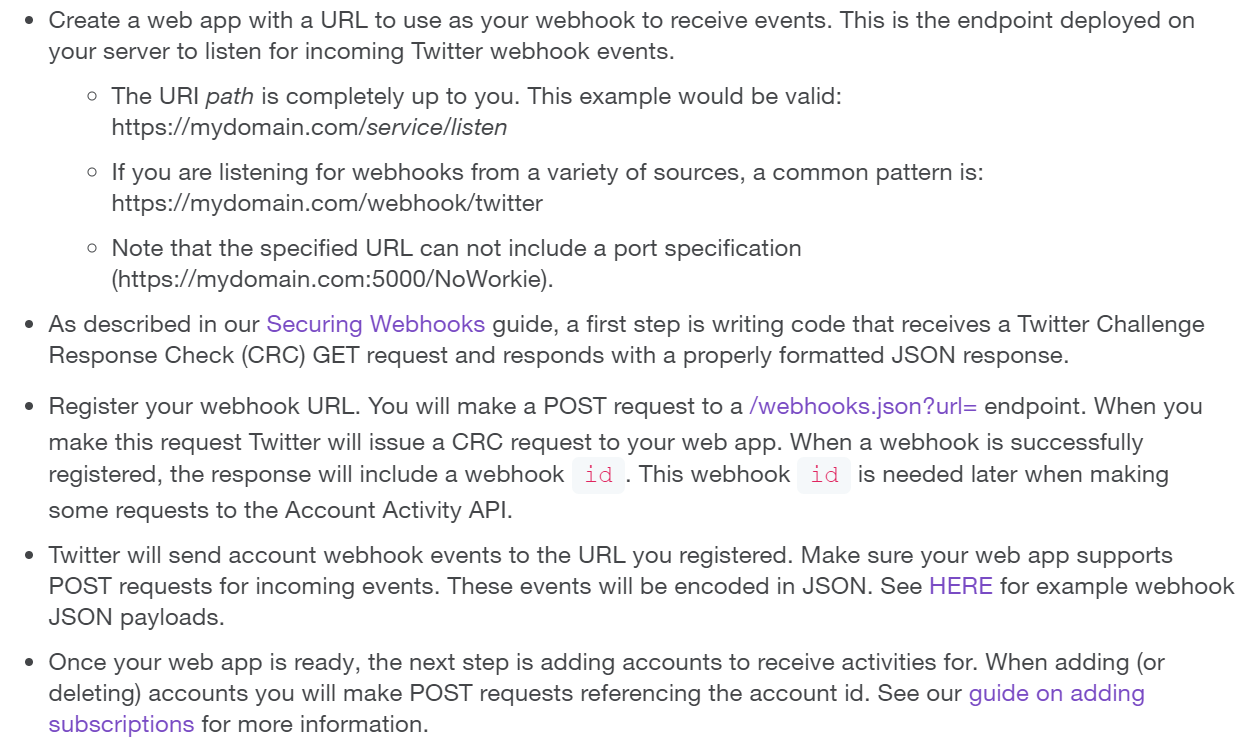
\includegraphics[width=1\linewidth]{images/accountActivitySteps}
		\caption{Steps to follow to implement a webhook connection with Twitter.}
		\label{accountActivitySteps}
		\end{figure}

		I created a web app with an URL to use my webhook to receive events (Figure 29). Everytime the app receives an event, it updates the internal list of tweets by using the 				getTweets function (this is limited to once per second to avoid spam and therefore avoid blacklisting of my account).

		\begin{figure}[H] % Example image
		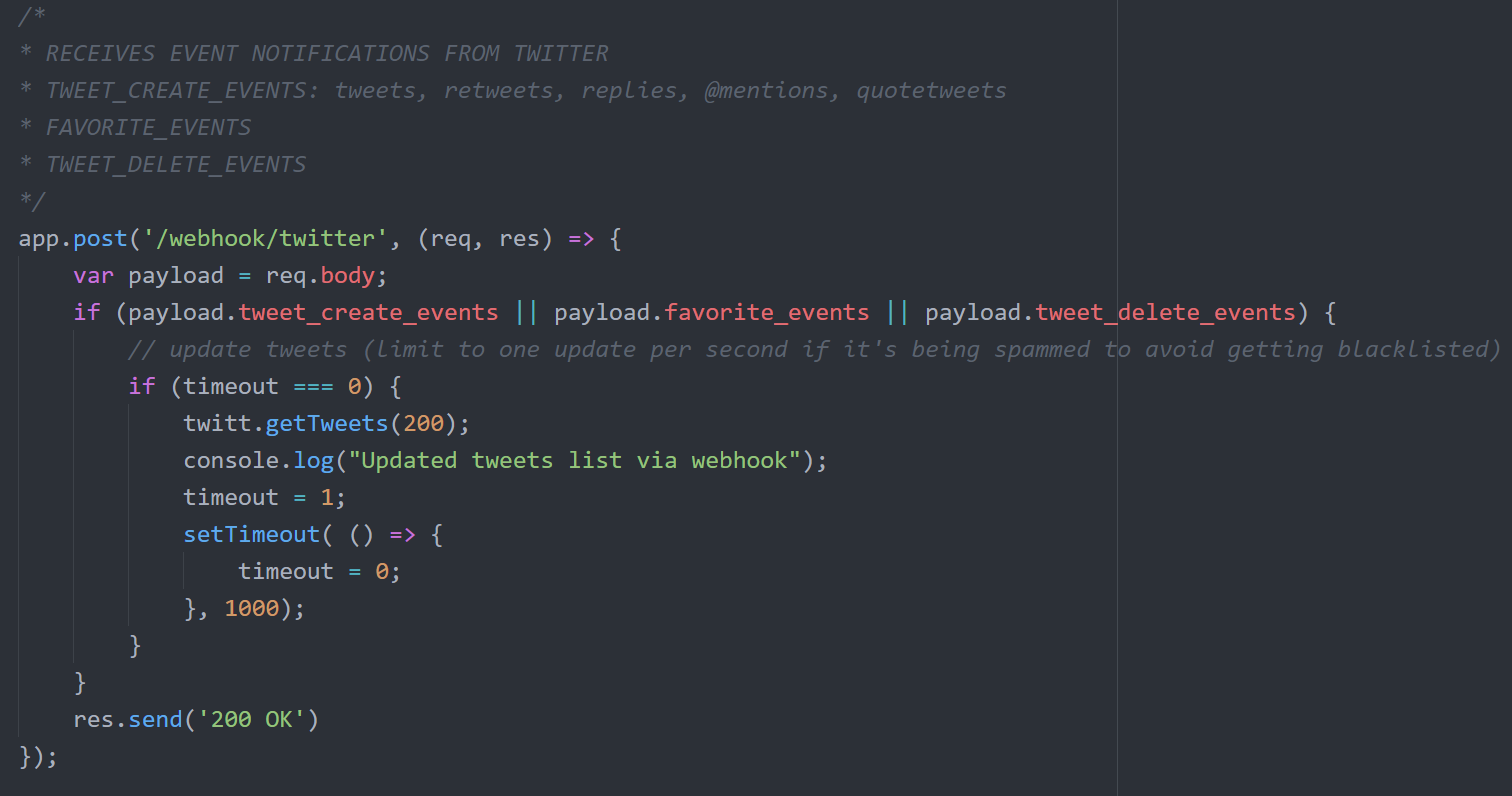
\includegraphics[width=1\linewidth]{images/webhookPOST}
		\caption{The app listens for POST requests on the specified URL, which refers to https://unimitwitterbot.herokuapp.com/webhook/twitter.}
		\label{webhookPOST}
		\end{figure}

		Then I implemented the code that resolves the Twitter Challenge Response Check: first of all we make a POST request to \url{/webhooks.json?url="myURL"} (Figure 30).
		According to Twitter, when a webhook is created they will issue a GET request with the CRC code and the app must respond with the requirements on Figure 31.
		The code that manages this GET request can be seen on Figure 32 and the code that creates the hash code on Figure 33.
		
		\begin{figure}[H] % Example image
		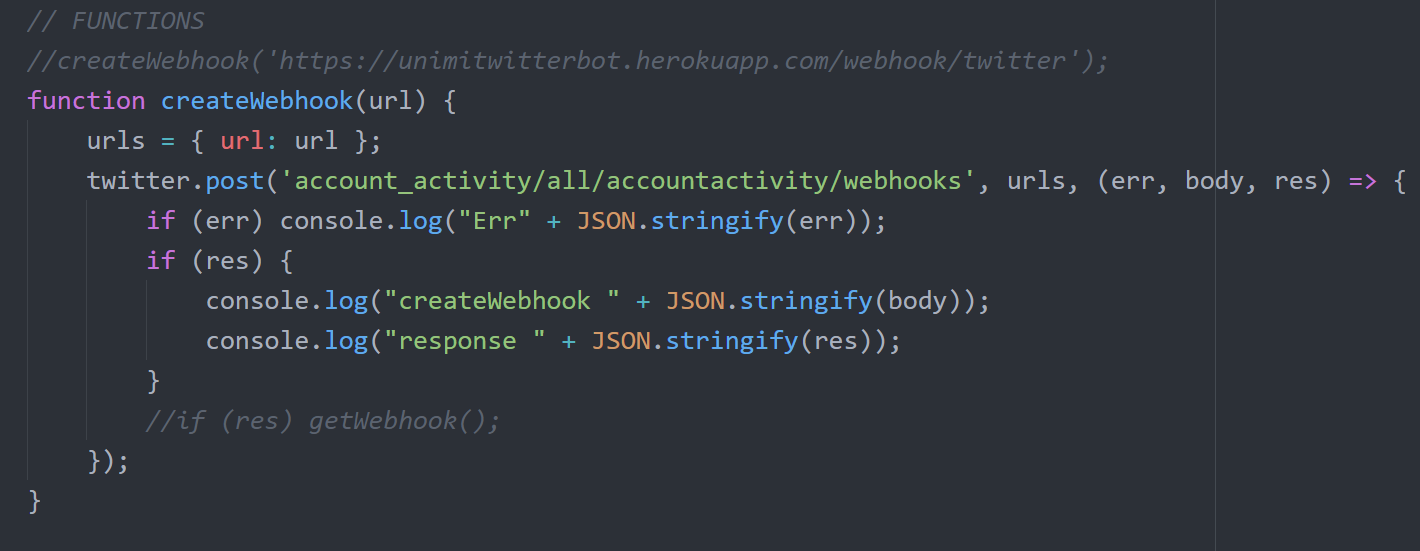
\includegraphics[width=1\linewidth]{images/createWebhook}
		\caption{Creating the webhook connection. Note that the commented out code was only executed once. The connection is persistent as long as we do atleast one
		validation a day.}
		\label{createWebhook}
		\end{figure}

		\begin{figure}[H] % Example image
		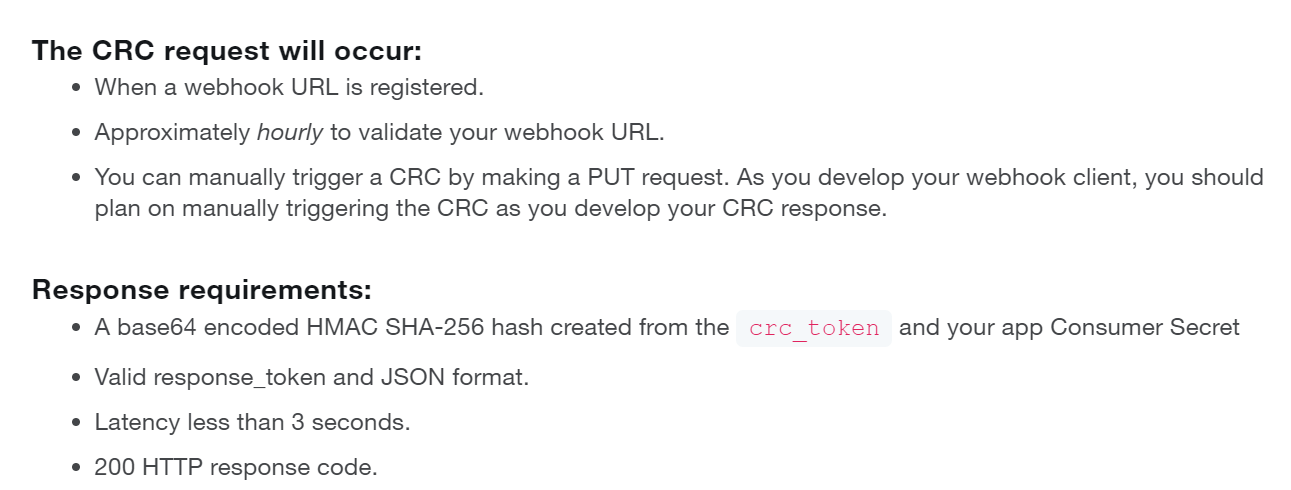
\includegraphics[width=1\linewidth]{images/CRCrequirements}
		\caption{CRC response requirements}
		\label{CRCrequirements}
		\end{figure}

		\begin{figure}[H] % Example image
		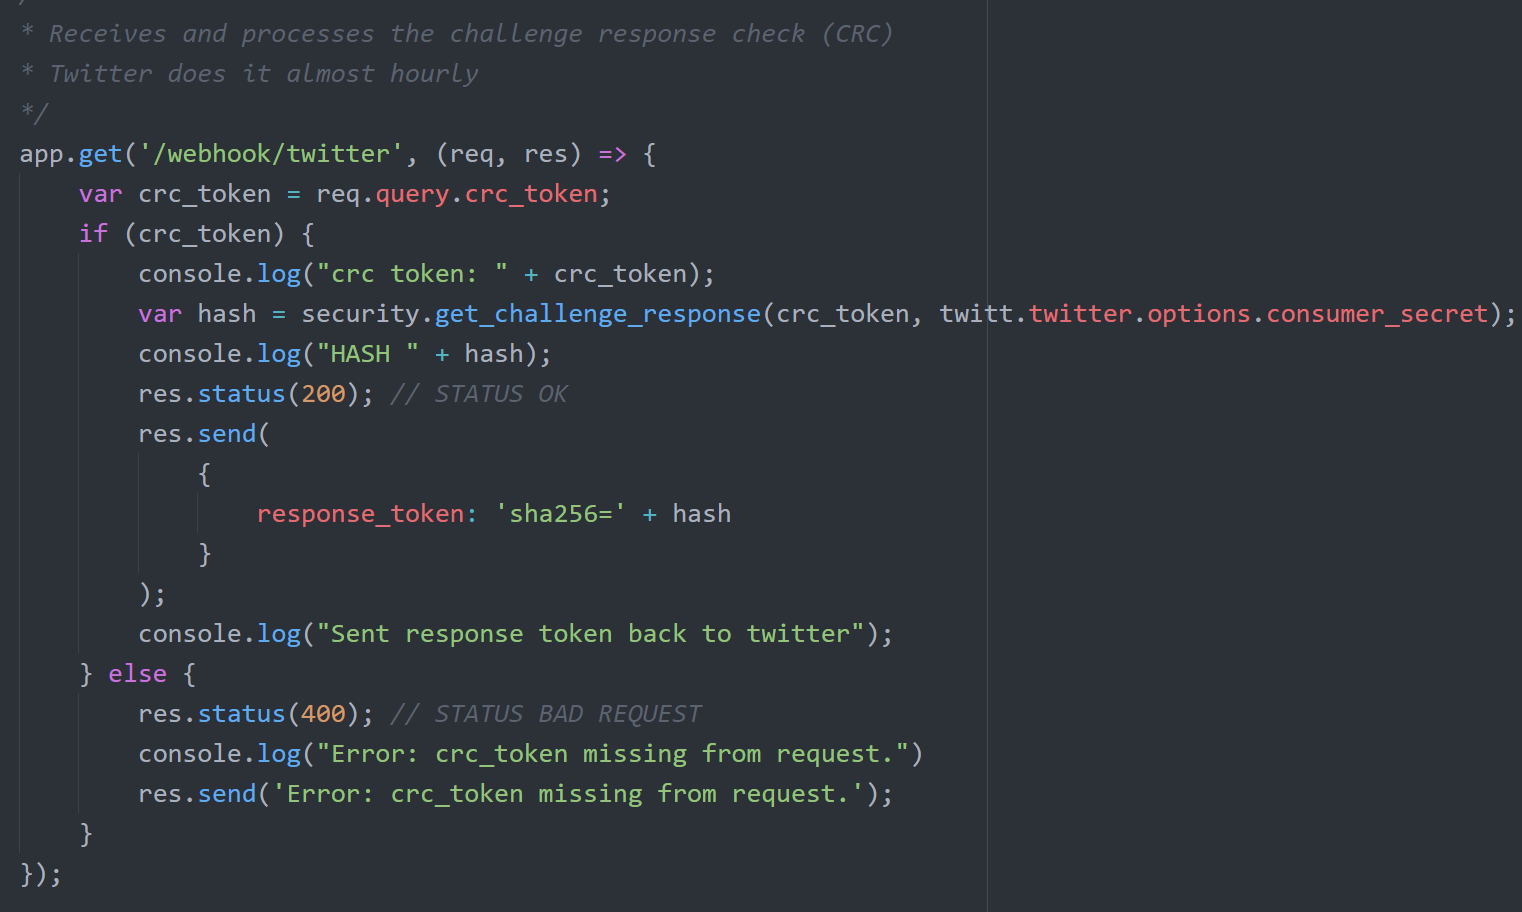
\includegraphics[width=1\linewidth]{images/CRCresponse}
		\caption{CRC response (code).}
		\label{CRCresponse}
		\end{figure}

		\begin{figure}[H] % Example image
		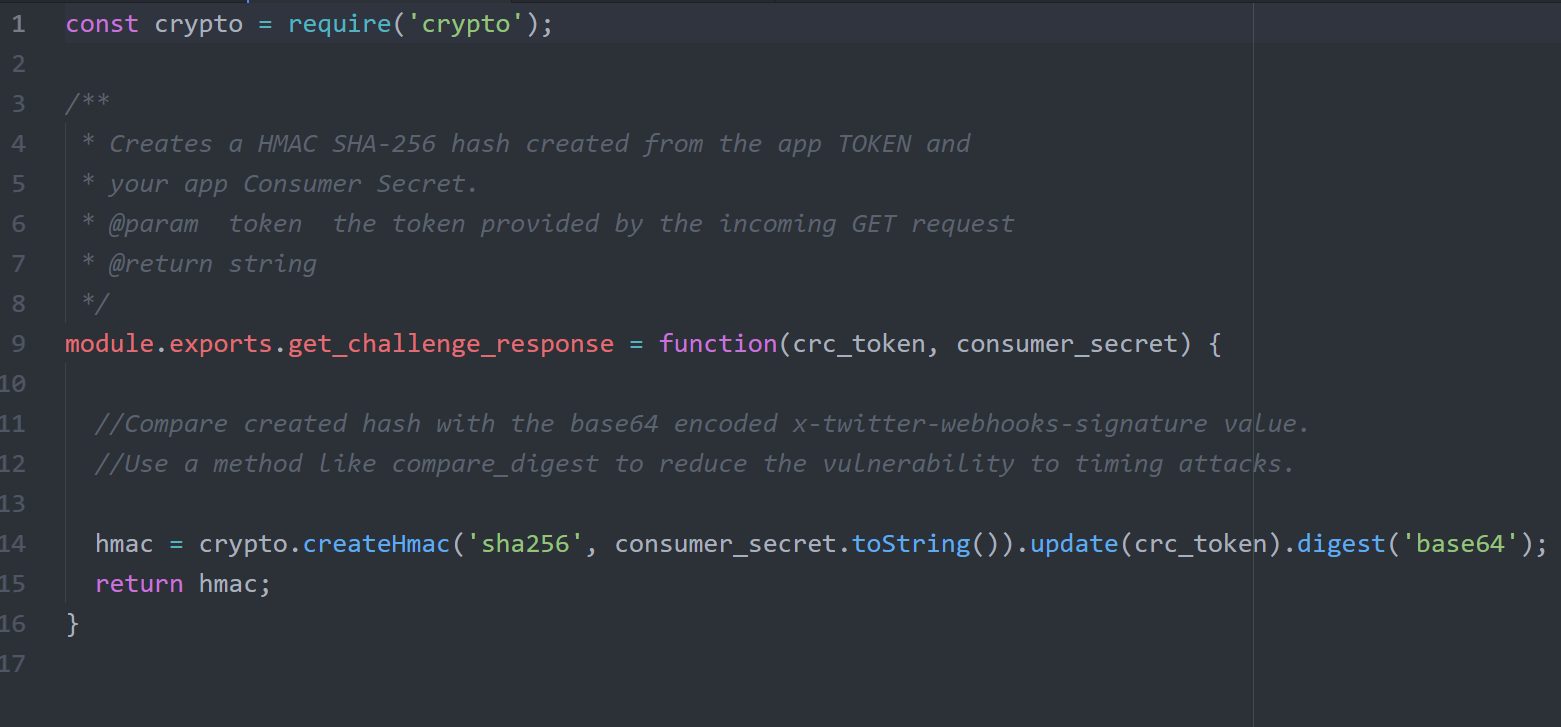
\includegraphics[width=1\linewidth]{images/hashCreation}
		\caption{Generating the hash code.}
		\label{hashCreation}
		\end{figure}

		The next step is registering a subscription for a certain user; in this case we register our own account (Figure 34). It's important to note that 
		we need user-supplied access tokens to do this so, for security reasons, we can't do this for any random account. 

		\begin{figure}[H] % Example image
		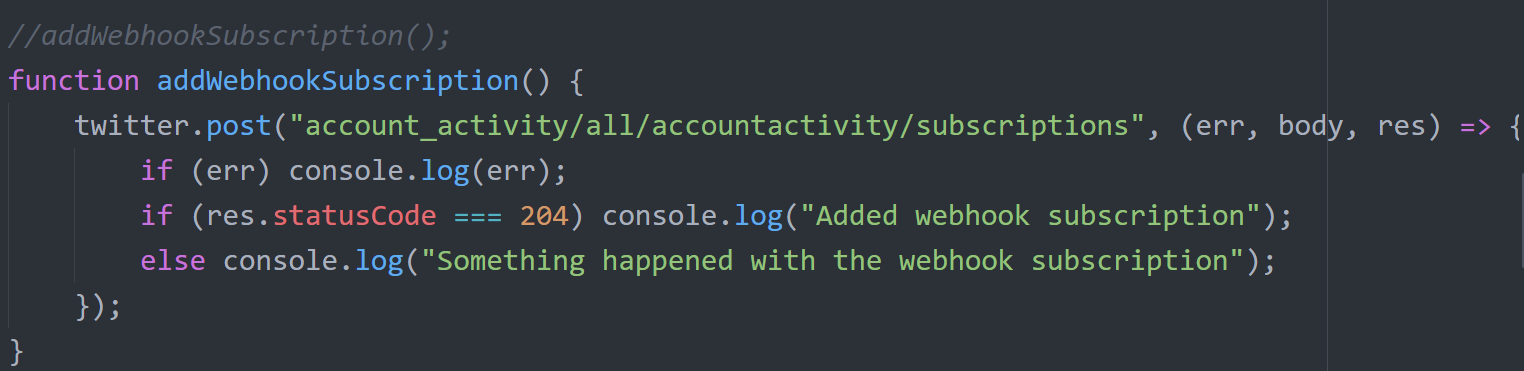
\includegraphics[width=1\linewidth]{images/addWebhookSubscription}
		\caption{Code to add webhook subscription with our own access token key. Remember that the OAuth is being managed by the twitter module (we created a twitter object 				with our own API keys}
		\label{addWebhookSubscription}
		\end{figure}

		The final step is testing the webhook: receiving events (Figure 29). An example of event is shown on Figure 35 after I favorited one of my own tweets.

		\begin{figure}[H] % Example image
		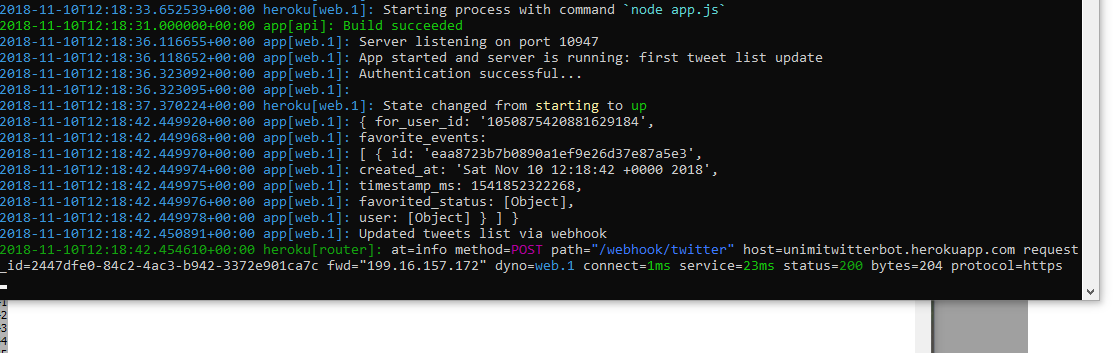
\includegraphics[width=1\linewidth]{images/favoriteEventExample}
		\caption{Example of a favorite\_event payload}
		\label{favoriteEventExample}
		\end{figure}

		Note that we use the webhooks in order to update our internal list of tweets (this way everytime an event happens, like a tweet or favorite event our list is updated).
		There's another, much simpler, way to do this but less efficient and it's based on updating the list every second. This means that we may make useless calls because
		the list won't change every second as opposed to update it every time something happens. This is how the app was implemented in the earlier stages and I still have the code
		but it's been commented out (Figure 36).

		\begin{figure}[H] % Example image
		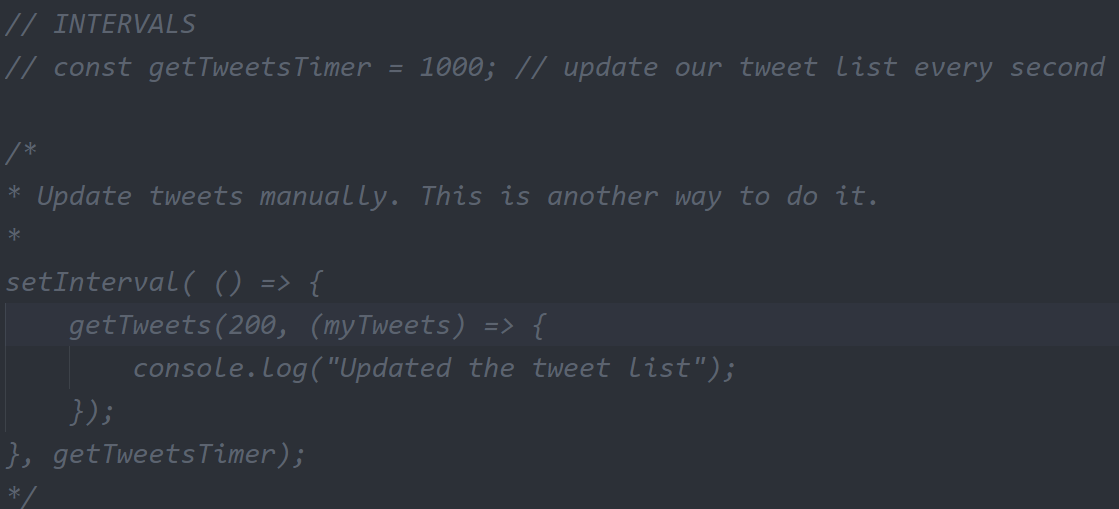
\includegraphics[width=1\linewidth]{images/intervalUpdate}
		\caption{Earlier implementation of the list update}
		\label{intervalUpdate}
		\end{figure}

	\end{enumerate}


%----------------------------------------------------------------------------------------
%	MAJOR SECTION 
%----------------------------------------------------------------------------------------

\section{Additional attachments} % Major section

\subsection{First Draft}

	\begin{figure}[H] % Example image
	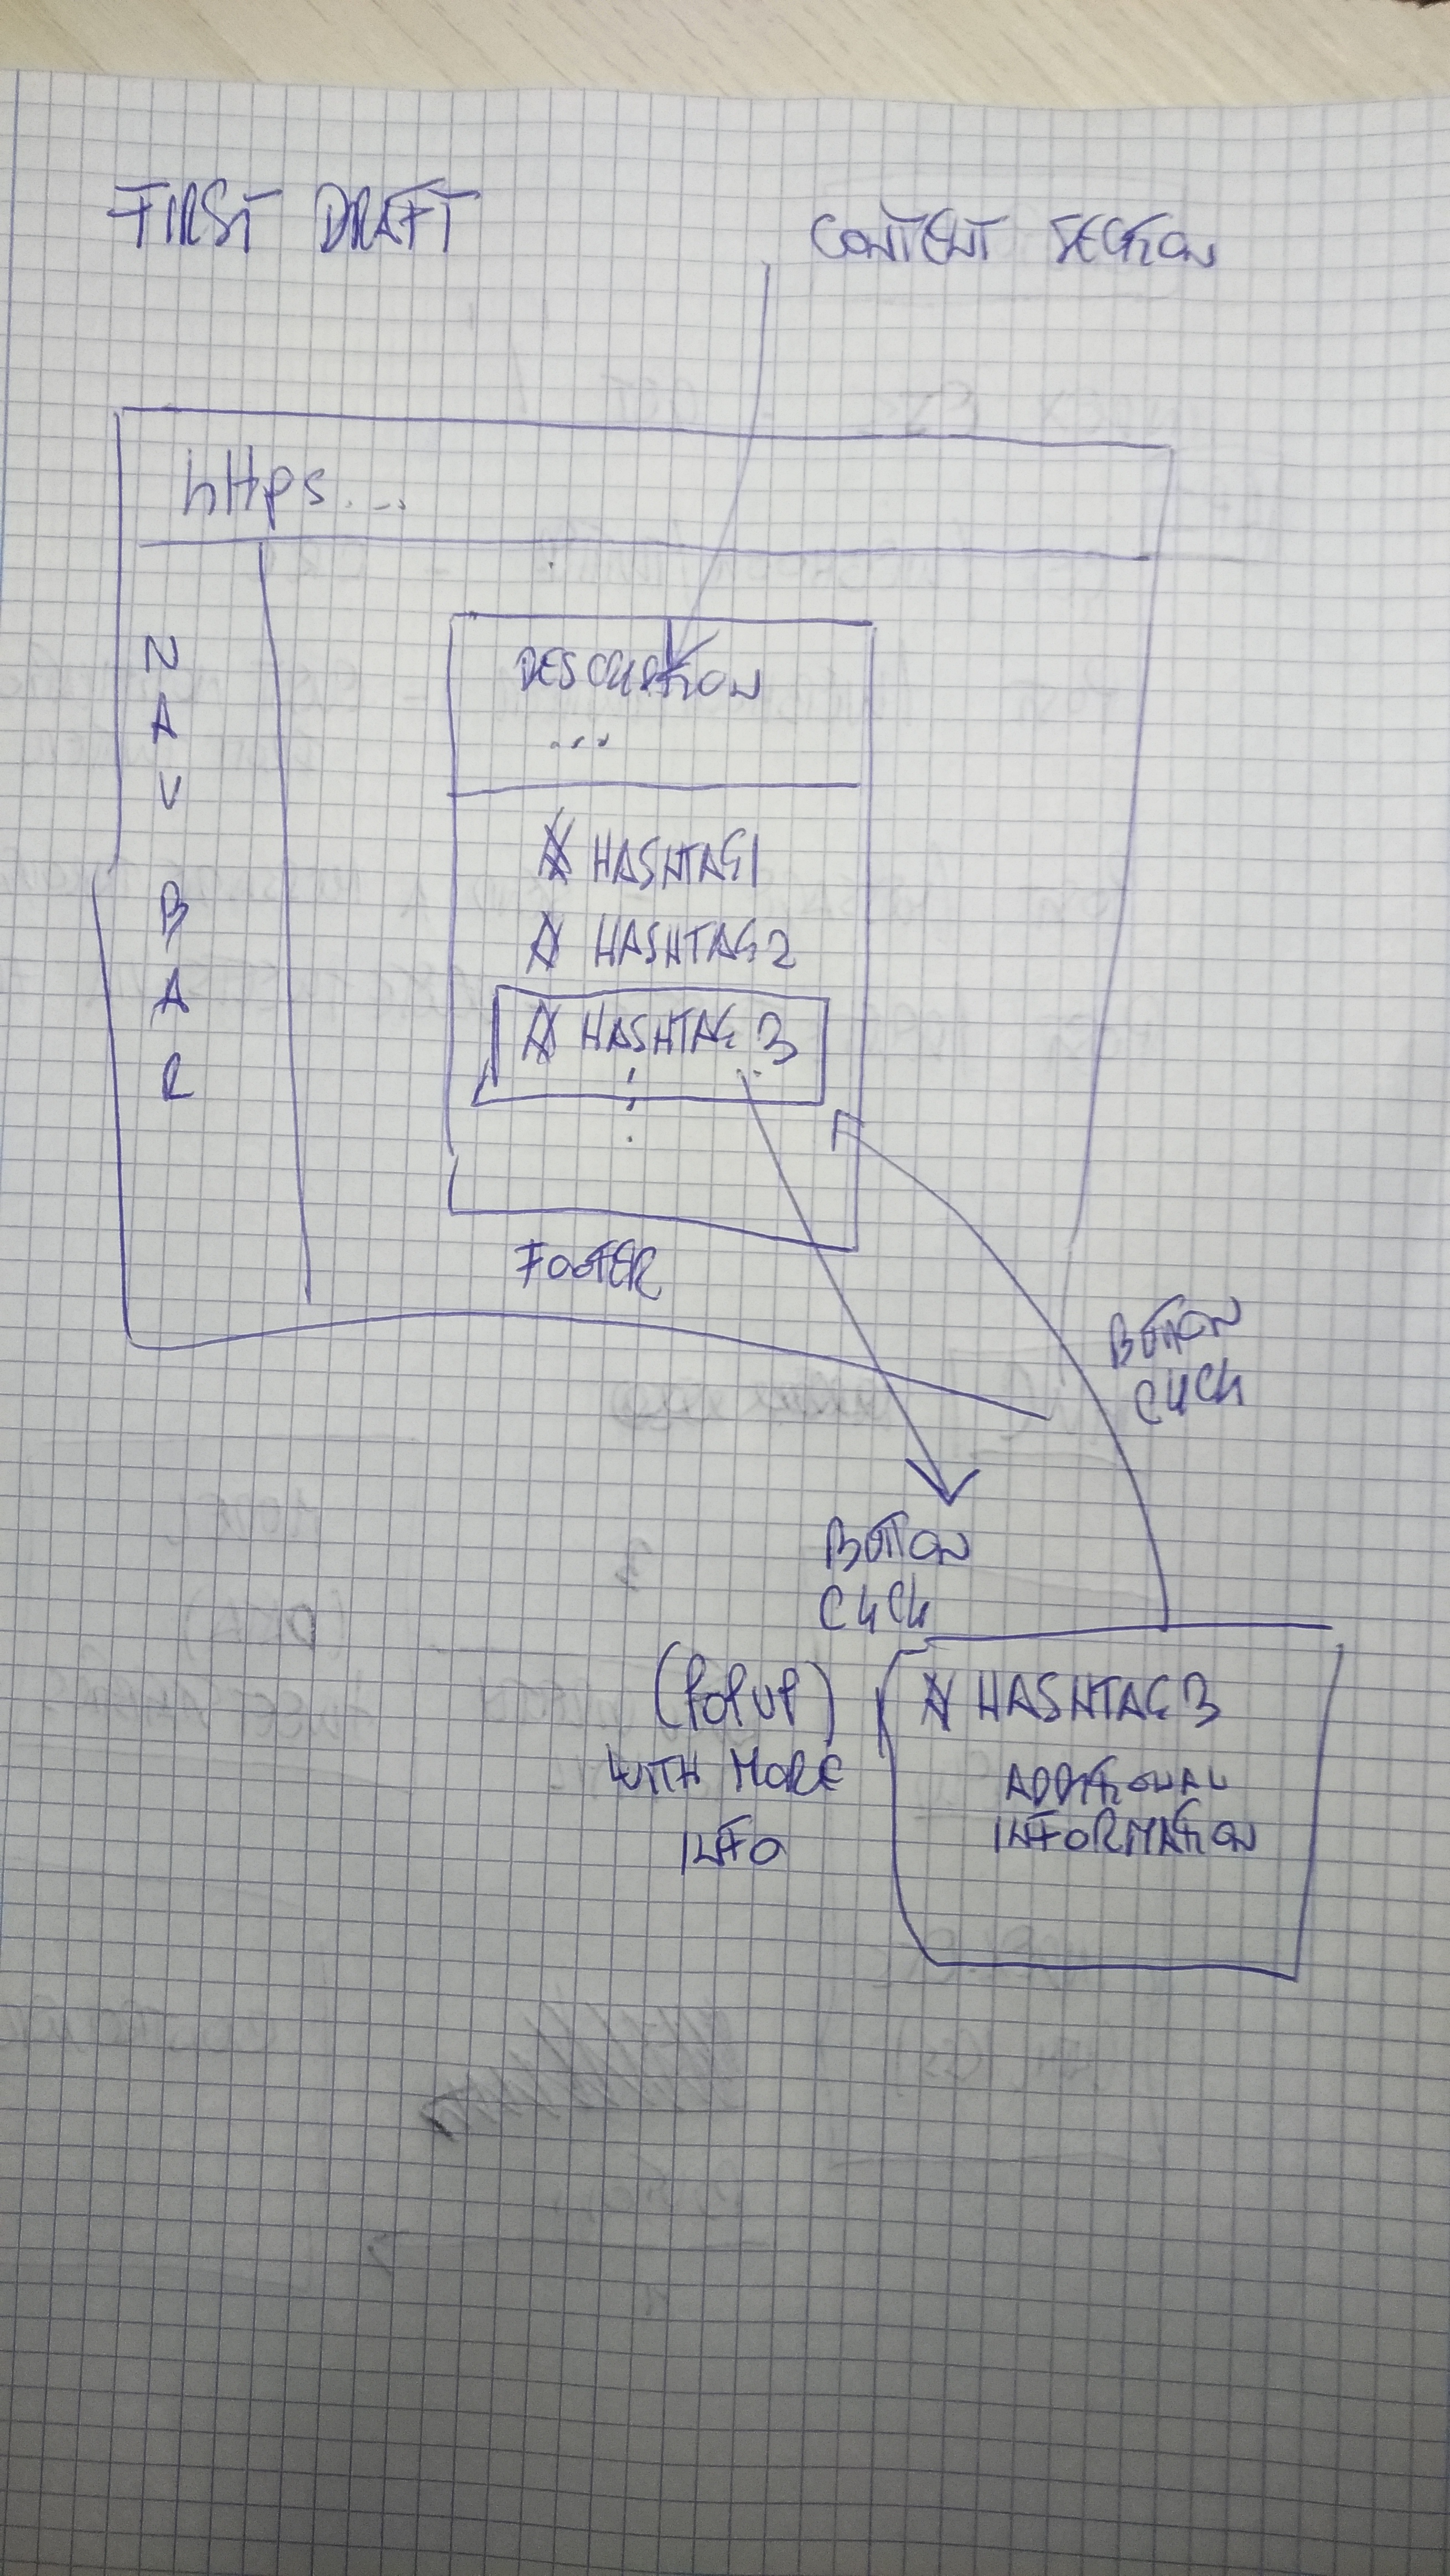
\includegraphics[width=0.6\linewidth]{images/first_draft}
	\caption{First draft of website}
	\label{firstDraft}
	\end{figure}

\subsection{Application API Endpoints}

	\begin{figure}[H] % Example image
	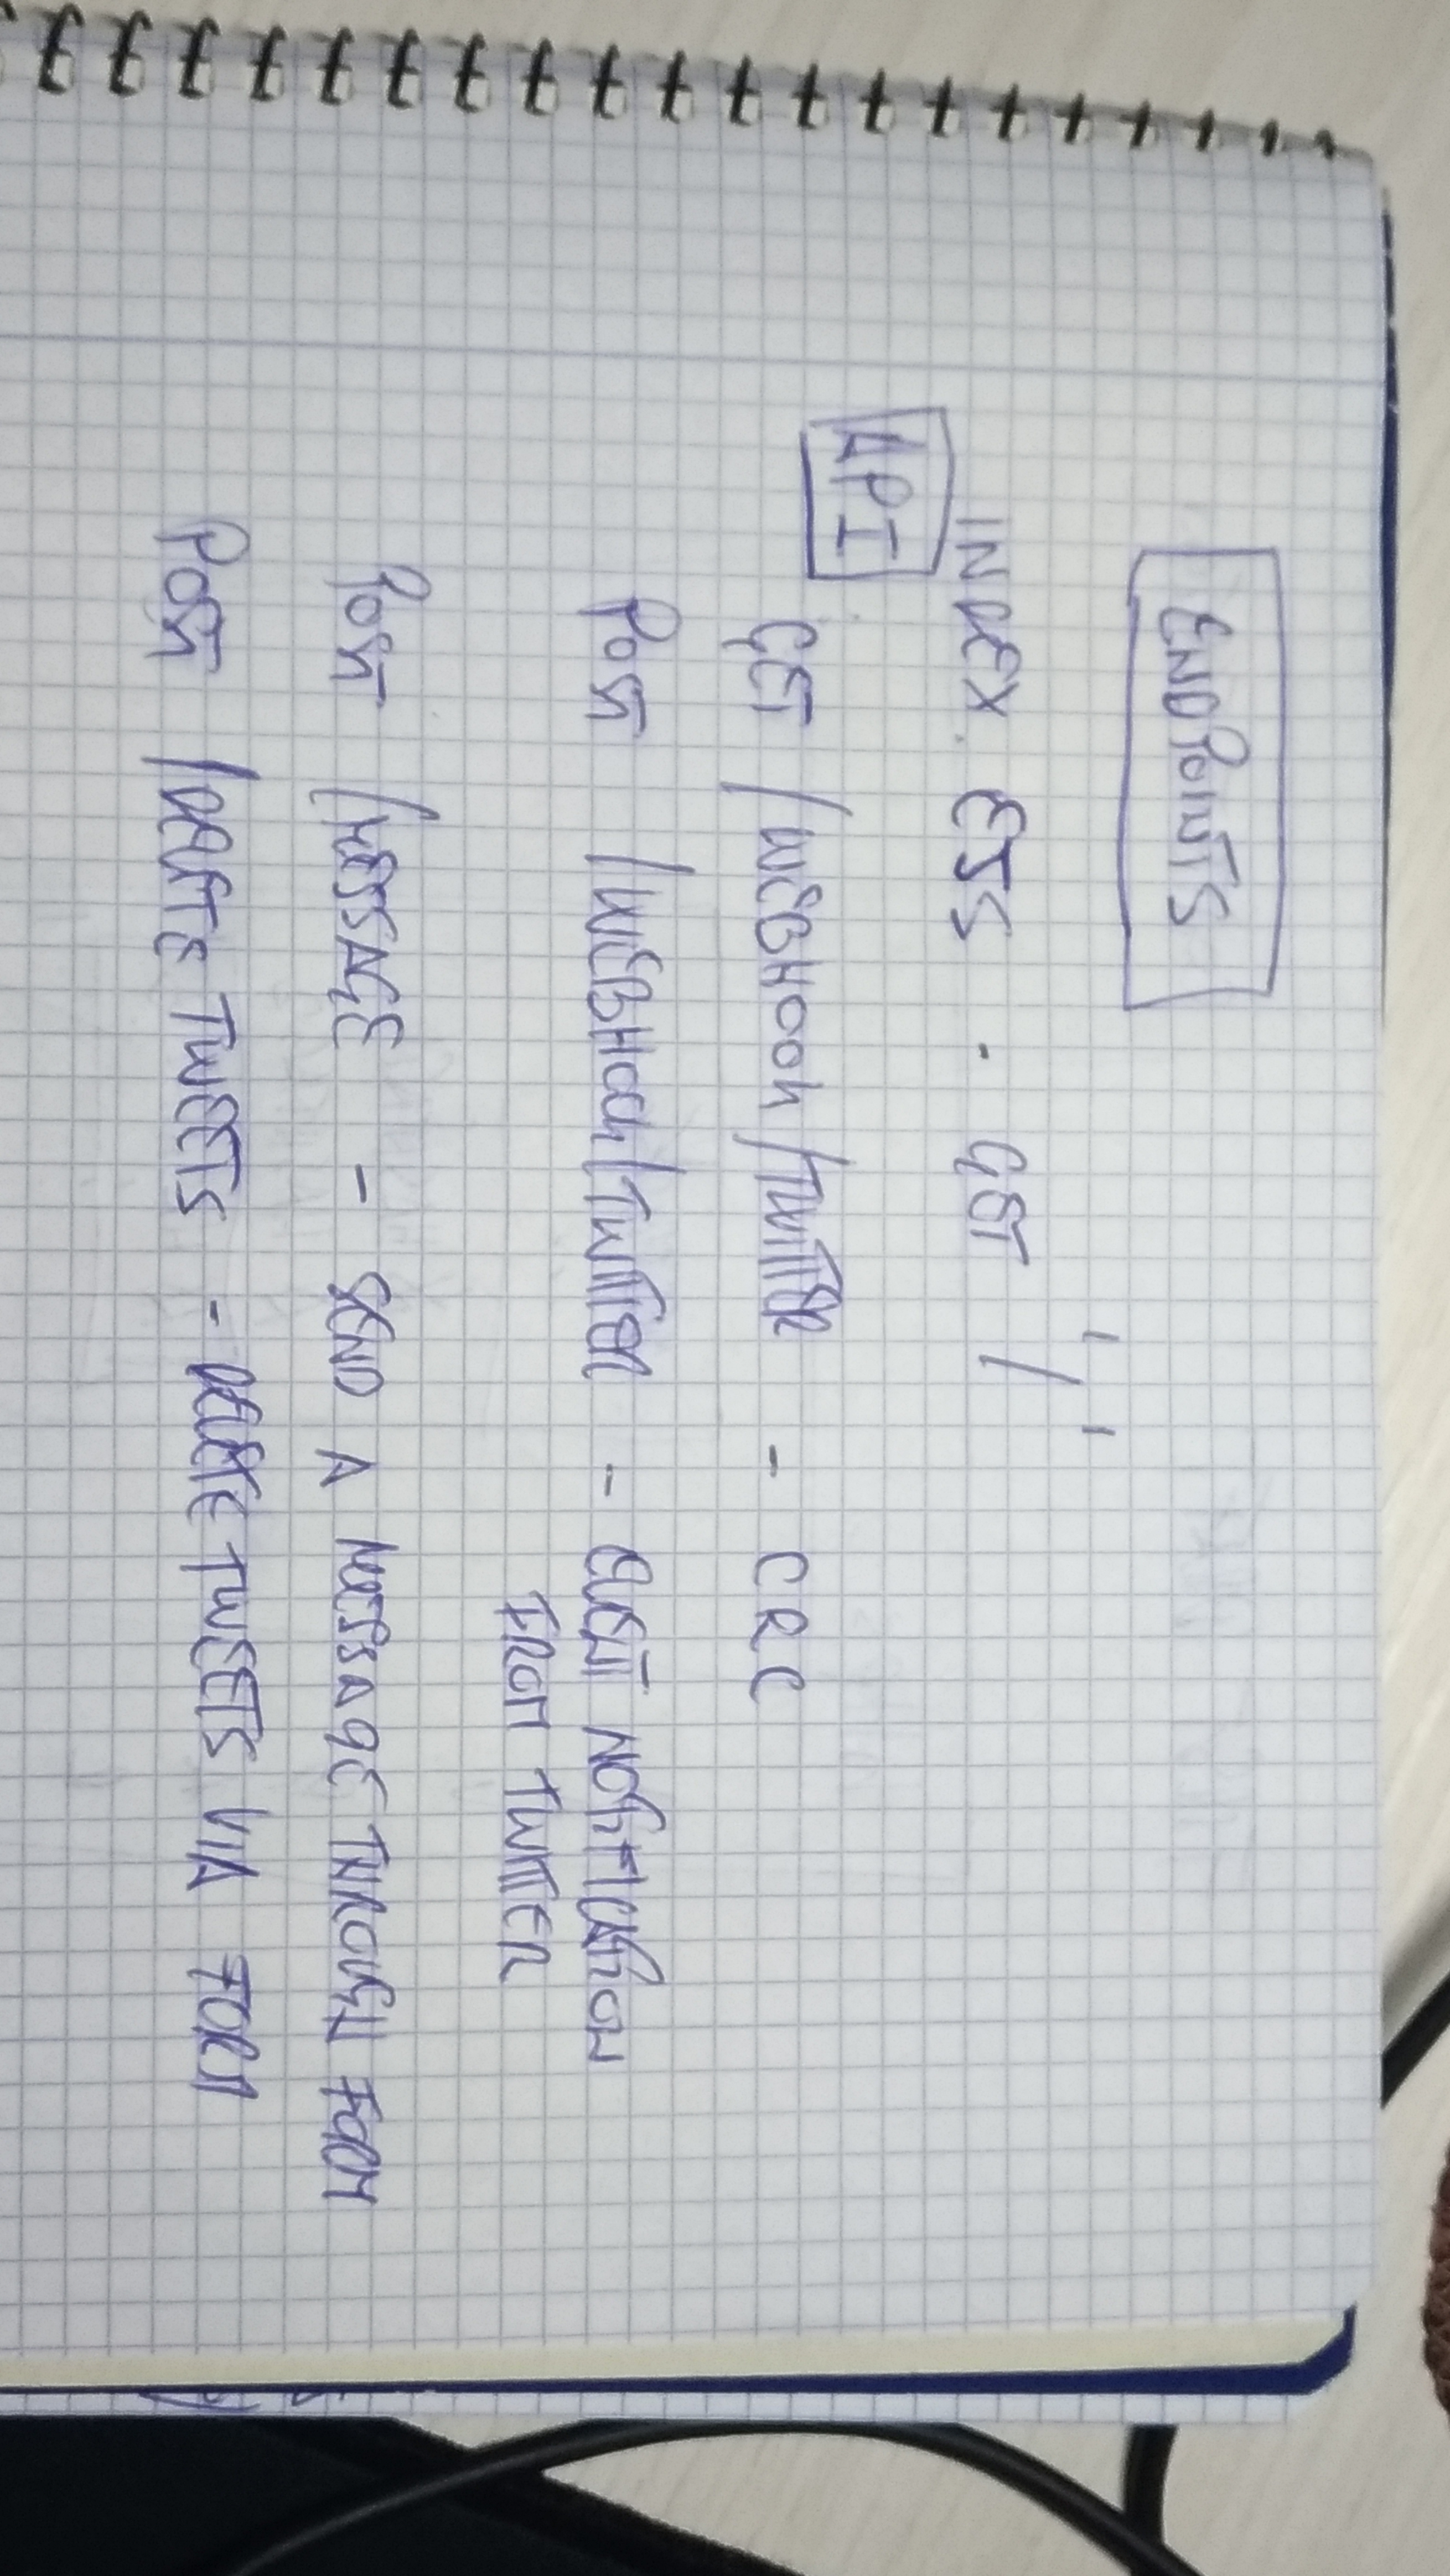
\includegraphics[width=0.7\linewidth]{images/API}
	\caption{API endpoints for application}
	\label{API)}
	\end{figure}

\subsection{MVC example}

	\begin{figure}[H] % Example image
	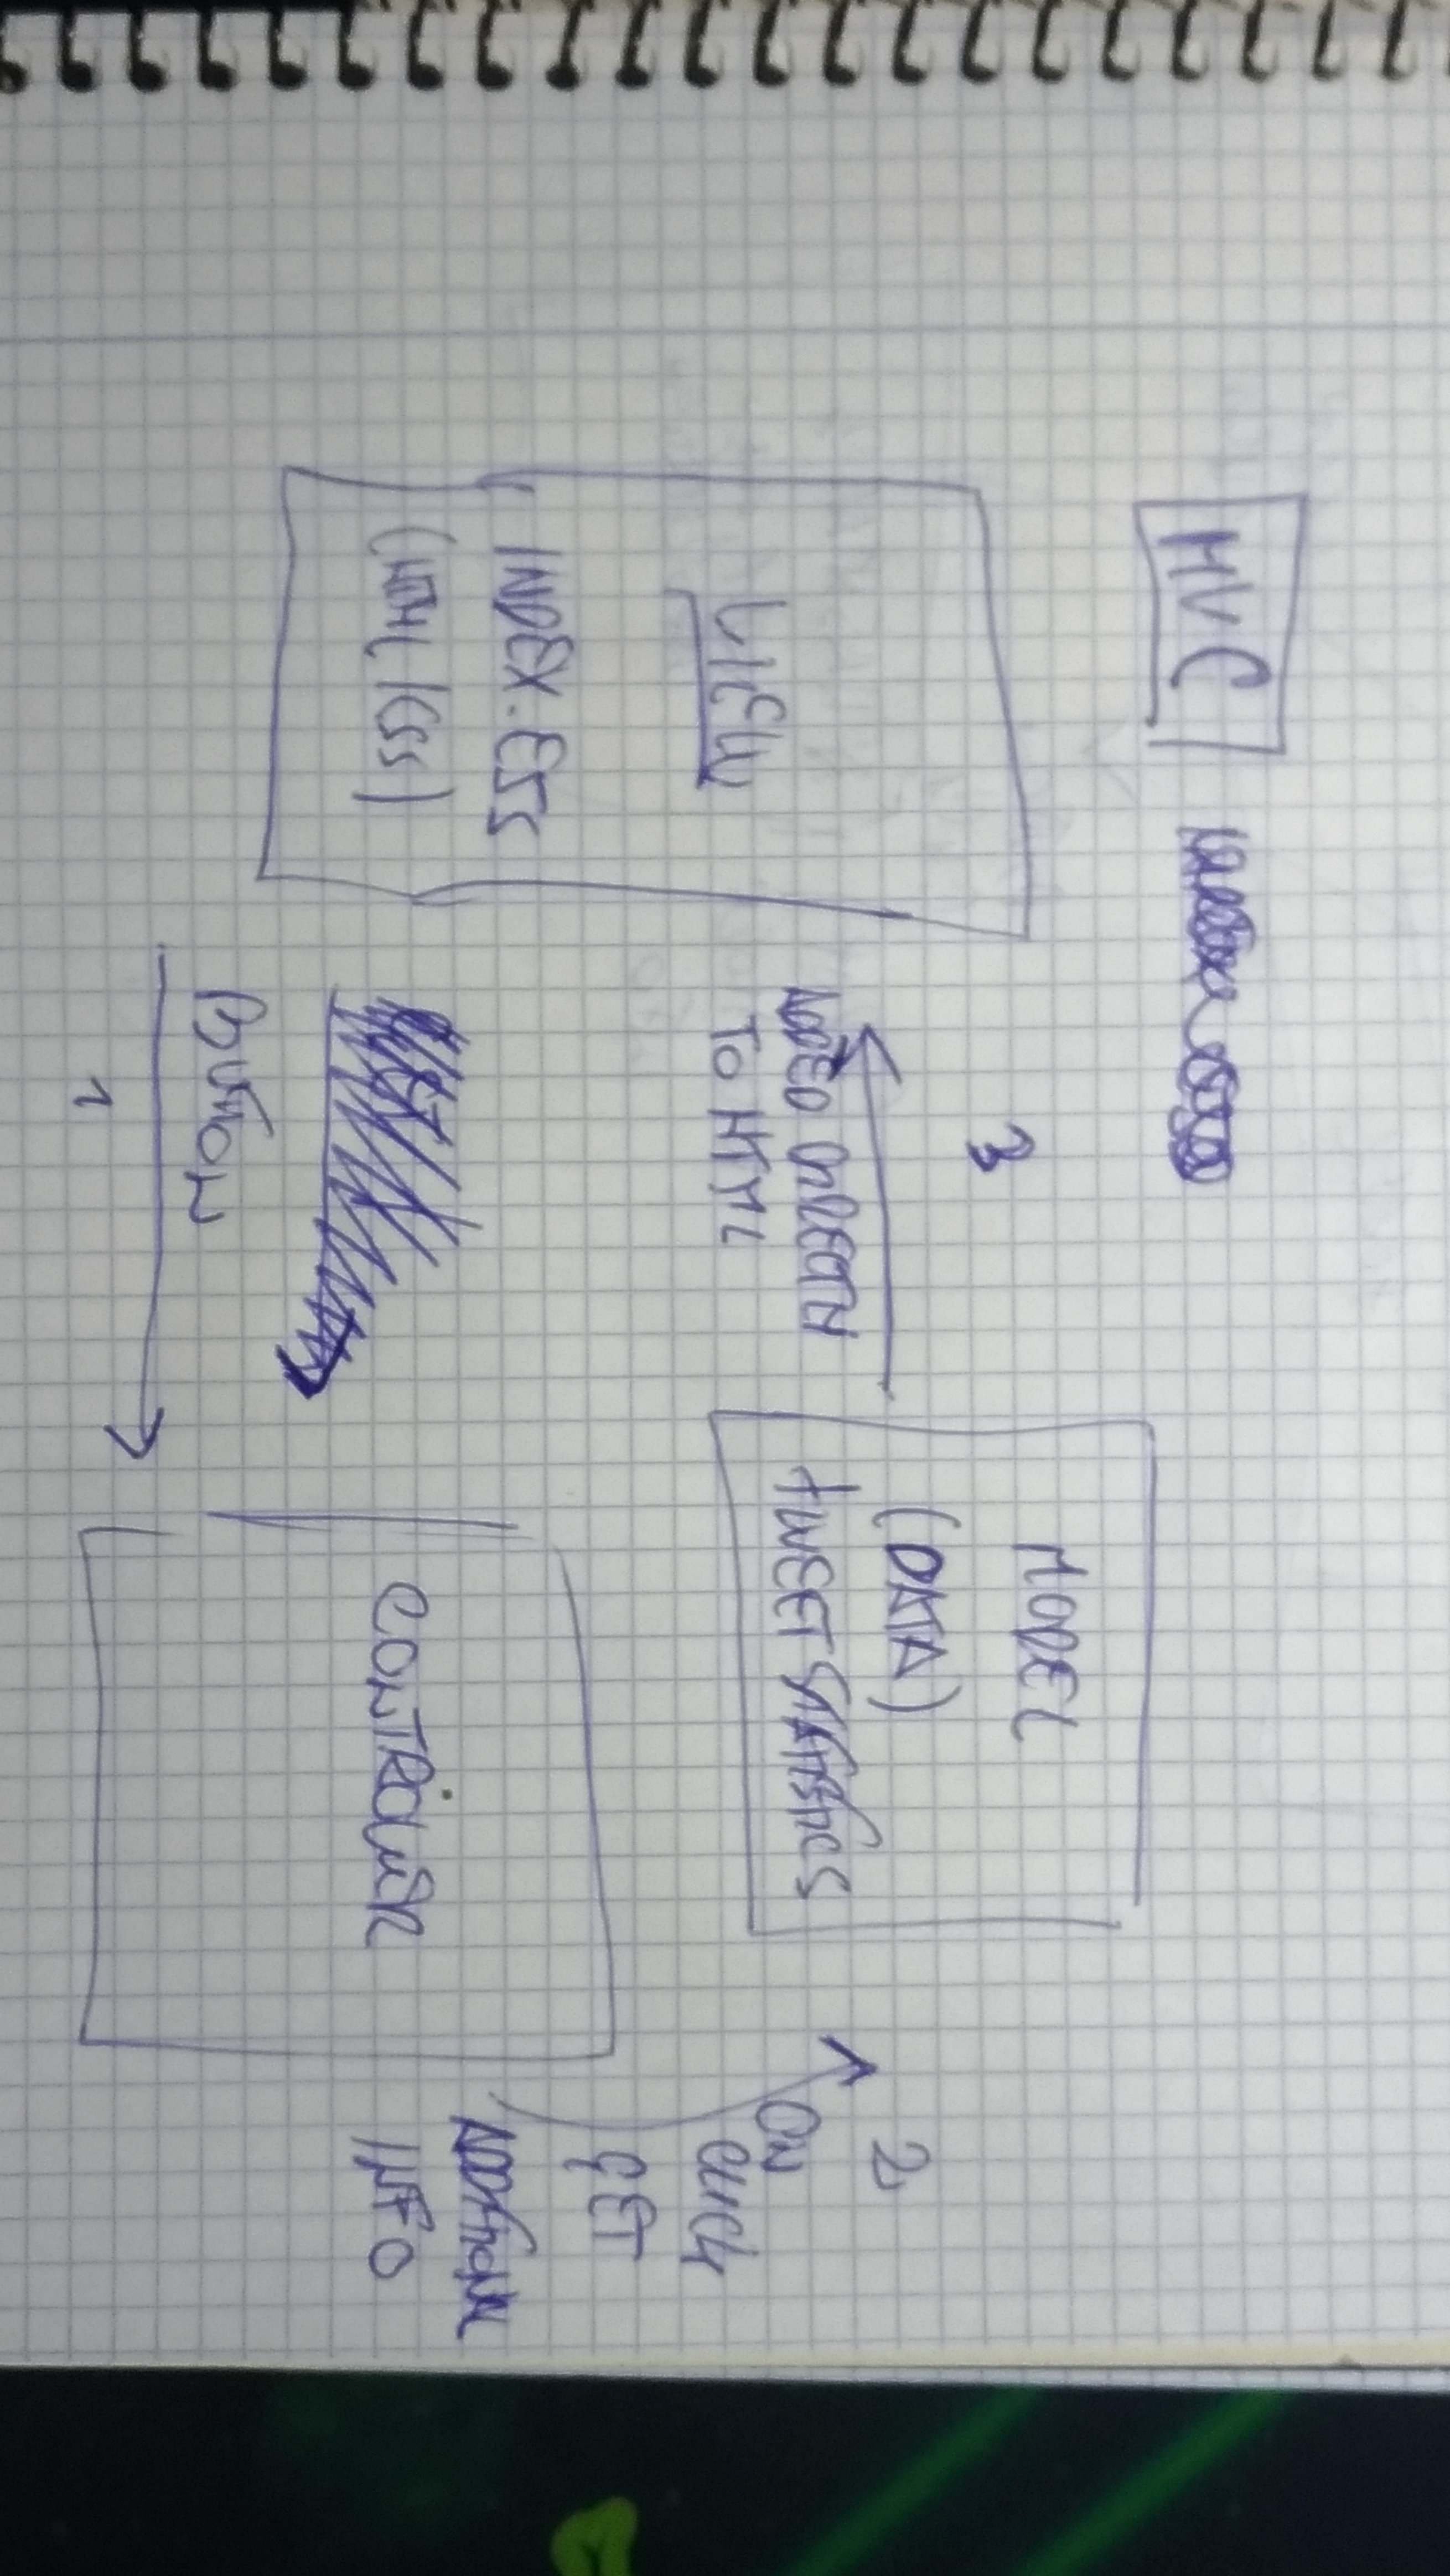
\includegraphics[width=0.7\linewidth]{images/MVC}
	\caption{MVC example for how the button click updates our view}
	\label{MVC)}
	\end{figure}

	

		
%----------------------------------------------------------------------------------------
%	CONCLUSION
%----------------------------------------------------------------------------------------

\section{Conclusion} % Major section

\noindent The purpose of this project was to get accustomed to some of the most important web development technologies such as HTML5, CSS (front-end), 
Javascript (front-end and back-end) and NodeJS (back-end). The app itself is not very useful to customers but it's not a commercial product and I only chose to do this project
in order to learn web development. 
It's taken me abouth a month to develop this app (including the project report which was written in LaTeX and was quite time consuming). All in all it was a good experience for me especially because I didn't know anything about web development beforehand and I quite like it and might pursue it further after graduating.

%----------------------------------------------------------------------------------------
%	BIBLIOGRAPHY
%----------------------------------------------------------------------------------------

\pagebreak

\bibliographystyle{unsrt}

\bibliography{references}

%----------------------------------------------------------------------------------------

\end{document}